
\documentclass[11pt]{article}

\usepackage[T1]{fontenc}
\usepackage[utf8]{inputenc}
\usepackage{lmodern}
\usepackage[a4paper,margin=1in]{geometry}
\usepackage{amsmath,amssymb,amsthm,mathtools,bm}
\usepackage{graphicx}
\usepackage{booktabs}
\usepackage{enumitem}
\usepackage{xcolor}
\usepackage{caption}
\usepackage{subcaption}
\usepackage{hyperref}
\usepackage[nameinlink,capitalise,noabbrev]{cleveref}
\usepackage{float}
\usepackage{setspace}
\usepackage{fancyhdr}
\usepackage{array}

\hypersetup{
  colorlinks=true,
  linkcolor=blue!55!black,
  citecolor=blue!55!black,
  urlcolor=blue!55!black,
  pdftitle={Diffusion on AR(1) Sequences},
  pdfauthor={OpenAI synthesis manuscript}
}

\setstretch{1.08}
\setlength{\parskip}{0.45em}
\setlength{\parindent}{0pt}
\setlength{\headheight}{14pt}
\allowdisplaybreaks
\numberwithin{equation}{section}

\pagestyle{fancy}
\fancyhf{}
\fancyhead[L]{Diffusion on AR(1) sequences}
\fancyhead[R]{\thepage}
\renewcommand{\headrulewidth}{0.4pt}

\newtheorem{theorem}{Theorem}[section]
\newtheorem{proposition}[theorem]{Proposition}
\newtheorem{lemma}[theorem]{Lemma}
\newtheorem{corollary}[theorem]{Corollary}
\theoremstyle{definition}
\newtheorem{definition}[theorem]{Definition}
\newtheorem{example}[theorem]{Example}
\theoremstyle{remark}
\newtheorem{remark}[theorem]{Remark}

\newcommand{\R}{\mathbb{R}}
\newcommand{\E}{\mathbb{E}}
\newcommand{\Var}{\operatorname{Var}}
\newcommand{\Cov}{\operatorname{Cov}}
\newcommand{\diag}{\operatorname{diag}}
\newcommand{\Id}{I}
\newcommand{\trans}{\mathsf{T}}
\newcommand{\diff}{\,\mathrm{d}}
\newcommand{\Ncal}{\mathcal{N}}
\newcommand{\norm}[1]{\lVert #1\rVert}
\newcommand{\inner}[2]{\langle #1,#2\rangle}

\title{\textbf{Diffusion on AR(1) Sequences:}\\
Joint Gaussian Structure, Precision Geometry, Spectral Decoupling, and Score Analysis}
\author{A self-contained mathematical synthesis manuscript}
\date{March 2026}

\begin{document}
\maketitle
\thispagestyle{empty}

\begin{abstract}
This manuscript gives a complete and self-contained mathematical treatment of a diffusion model applied to a Gaussian AR(1) sequence. The target object is a trajectory of correlated frames, and the guiding question is how the Markov structure of the clean process is encoded in the score and how that structure is reshaped by diffusion noise. We proceed from first principles. We define the clean stochastic process, derive its mean, variance, and covariance by explicit recursion unrolling, compare stationary and non-stationary regimes, and analyze the three stability cases $|\alpha|<1$, $|\alpha|=1$, and $|\alpha|>1$. We then derive the full joint clean law, write it as a Gaussian quadratic form, and compute the tridiagonal precision matrix explicitly.

Next, we define the framewise Ornstein--Uhlenbeck forward diffusion, construct the conditional, joint, and marginal noisy laws, and derive the noisy covariance
\[
\Sigma_t = e^{-2t}\Sigma_0 + \Delta_t \Id,
\qquad
\Delta_t = 1-e^{-2t},
\]
by two independent methods: direct covariance calculation and Gaussian closure under affine transformations. This yields the exact score
\[
S(\mathbf{x},t)=\nabla_{\mathbf{x}}\log P_t(\mathbf{x})=-\Sigma_t^{-1}(\mathbf{x}-\boldsymbol{\mu}_t).
\]

The second half of the manuscript studies the structure of $\Sigma_t$ and $\Sigma_t^{-1}$. We prove the spectral theorem for real symmetric matrices, show that $\Sigma_0$ is symmetric positive definite, diagonalize it as $\Sigma_0=U\Lambda U^\trans$, and prove that the same orthogonal basis diagonalizes $\Sigma_t$ for every diffusion time. This yields full modewise decoupling in the eigenbasis, where each coordinate is an independent scalar Gaussian denoising problem. We then rewrite the precision in signal-to-noise ratio form,
\[
\Sigma_t^{-1} = \frac{1}{\Delta_t}(\Id+\gamma_t\Sigma_0)^{-1},
\qquad
\gamma_t = \frac{e^{-2t}}{\Delta_t},
\]
and interpret the loss of sparsity, the flattening of the spectrum, the improvement of conditioning, and the transition from local Markov structure to isotropic noise. Numerical figures are generated from reproducible scripts bundled with the project. The exposition synthesizes and unifies the derivations and structural insights developed in the companion notes on AR(1) diffusion, score structure, and spectral analysis \cite{draftar1,structure,anatomy,companion,mezardnotes,biroli2023}.
\end{abstract}

\newpage
\tableofcontents
\newpage

\section{Problem formulation}\label{sec:problem}

We formalize the stochastic process to be studied and fix notation.

\begin{definition}[Dynamic object, internal time, clean trajectory]
A \emph{dynamic object} is a finite trajectory
\[
\mathbf{a}=(a_0,a_1,\dots,a_K)^\trans\in\R^{K+1}.
\]
The index set $\{0,1,\dots,K\}$ is the \emph{internal time axis}; the individual random variables $a_k$ are the \emph{clean frames}. We set
\[
N:=K+1
\]
for the trajectory dimension.
\end{definition}

\begin{definition}[AR(1) process]
Fix parameters
\[
\mu_0\in\R,\qquad \sigma_0^2>0,\qquad \sigma_\eta^2>0,\qquad \alpha\in\R.
\]
The clean process is defined recursively by
\begin{equation}\label{eq:ar1_recursion}
a_{k+1}=\alpha a_k+\eta_k,\qquad k=0,1,\dots,K-1,
\end{equation}
with initial condition
\begin{equation}\label{eq:a0_law}
a_0\sim \Ncal(\mu_0,\sigma_0^2),
\end{equation}
and innovation sequence
\begin{equation}\label{eq:innovations}
\eta_k \stackrel{\mathrm{i.i.d.}}{\sim}\Ncal(0,\sigma_\eta^2).
\end{equation}
\end{definition}

\begin{definition}[Transition kernel]
The transition kernel induced by \eqref{eq:ar1_recursion} is
\begin{equation}\label{eq:transition_kernel}
M(a_{k+1}\mid a_k)
=
\frac{1}{\sqrt{2\pi\sigma_\eta^2}}
\exp\!\left[-\frac{(a_{k+1}-\alpha a_k)^2}{2\sigma_\eta^2}\right].
\end{equation}
\end{definition}

\begin{definition}[Independence assumptions]
The model satisfies the following assumptions.
\begin{enumerate}[label=(\roman*),leftmargin=1.2cm]
\item $a_0$ is independent of every innovation $\eta_k$;
\item the innovations $(\eta_0,\eta_1,\dots,\eta_{K-1})$ are independent and identically distributed;
\item the process is first-order Markov:
\[
p(a_{k+1}\mid a_k,a_{k-1},\dots,a_0)=p(a_{k+1}\mid a_k).
\]
\end{enumerate}
\end{definition}

\begin{remark}[Interpretation]
The AR(1) process is the simplest Gaussian model carrying genuine temporal structure. The coefficient $\alpha$ controls memory, the innovations inject fresh randomness, and the Markov property says that once the present frame $a_k$ is known, the earlier past is irrelevant for predicting $a_{k+1}$. The whole trajectory is therefore a correlated Gaussian object with a local conditional dependence structure.
\end{remark}

\section{Clean process analysis}\label{sec:clean}

We derive the full first- and second-order structure of the clean trajectory directly from the recursion.

\subsection{Basic definitions and algebraic identities}

\begin{definition}[Mean, variance, covariance]
For square-integrable random variables $X$ and $Y$:
\[
\E[X] \text{ is the mean},\qquad
\Var(X):=\E[(X-\E[X])^2],\qquad
\Cov(X,Y):=\E[(X-\E[X])(Y-\E[Y])].
\]
\end{definition}

\begin{lemma}[Linearity of expectation]\label{lem:linexp}
For any square-integrable random variables $X,Y$ and scalars $a,b\in\R$,
\[
\E[aX+bY]=a\E[X]+b\E[Y].
\]
\end{lemma}

\begin{proof}
By the linearity of the integral,
\[
\E[aX+bY]=\int (aX+bY)\diff\mathbb P
=a\int X\diff\mathbb P+b\int Y\diff\mathbb P
=a\E[X]+b\E[Y].
\]
\end{proof}

\begin{lemma}[Variance of an affine transformation]\label{lem:var_affine}
For every square-integrable random variable $X$ and every $a,b\in\R$,
\[
\Var(aX+b)=a^2\Var(X).
\]
\end{lemma}

\begin{proof}
Using the definition of variance and \Cref{lem:linexp},
\begin{align*}
\Var(aX+b)
&=\E\!\left[\big((aX+b)-\E[aX+b]\big)^2\right] \\
&=\E\!\left[\big(aX+b-(a\E[X]+b)\big)^2\right] \\
&=\E\!\left[a^2(X-\E[X])^2\right] \\
&=a^2\Var(X).
\end{align*}
\end{proof}

\begin{lemma}[Variance of a sum]\label{lem:var_sum}
For square-integrable $X,Y$,
\[
\Var(X+Y)=\Var(X)+\Var(Y)+2\Cov(X,Y).
\]
In particular, if $X$ and $Y$ are independent, then
\[
\Var(X+Y)=\Var(X)+\Var(Y).
\]
\end{lemma}

\begin{proof}
Expand the square:
\begin{align*}
\Var(X+Y)
&=\E\!\left[\big((X-\E[X])+(Y-\E[Y])\big)^2\right] \\
&=\E[(X-\E[X])^2]+\E[(Y-\E[Y])^2] \\
&\quad +2\E[(X-\E[X])(Y-\E[Y])] \\
&=\Var(X)+\Var(Y)+2\Cov(X,Y).
\end{align*}
If $X$ and $Y$ are independent, then $\E[XY]=\E[X]\E[Y]$, hence $\Cov(X,Y)=0$.
\end{proof}

\begin{lemma}[Independent variables have zero covariance]\label{lem:cov_zero}
If $X$ and $Y$ are independent and square-integrable, then
\[
\Cov(X,Y)=0.
\]
\end{lemma}

\begin{proof}
By definition,
\[
\Cov(X,Y)=\E[XY]-\E[X]\E[Y].
\]
Independence gives $\E[XY]=\E[X]\E[Y]$, so the difference is zero.
\end{proof}

\begin{lemma}[Measurable functions of independent families remain independent]\label{lem:meas_func_indep}
Let $U$ and $V$ be independent random elements and let $f,g$ be measurable. Then $f(U)$ and $g(V)$ are independent.
\end{lemma}

\begin{proof}
For any Borel sets $A$ and $B$,
\[
\{f(U)\in A\}=\{U\in f^{-1}(A)\},
\qquad
\{g(V)\in B\}=\{V\in g^{-1}(B)\}.
\]
Hence
\begin{align*}
\mathbb P(f(U)\in A,\ g(V)\in B)
&=\mathbb P(U\in f^{-1}(A),\,V\in g^{-1}(B)) \\
&=\mathbb P(U\in f^{-1}(A))\,\mathbb P(V\in g^{-1}(B)) \\
&=\mathbb P(f(U)\in A)\,\mathbb P(g(V)\in B).
\end{align*}
\end{proof}

\begin{lemma}[Finite geometric series]\label{lem:geom}
For any scalar $r\neq 1$ and integer $k\geq 1$,
\[
\sum_{j=0}^{k-1}r^j = \frac{1-r^k}{1-r}.
\]
\end{lemma}

\begin{proof}
Set
\[
S_k:=1+r+r^2+\cdots+r^{k-1}.
\]
Multiply by $r$:
\[
rS_k = r+r^2+\cdots+r^k.
\]
Subtract the two identities:
\[
S_k-rS_k = 1-r^k.
\]
Factor:
\[
(1-r)S_k=1-r^k.
\]
Because $r\neq 1$, division by $1-r$ gives the result.
\end{proof}

\subsection{Explicit unrolling of the recursion}

\begin{proposition}[Unrolled form of the clean trajectory]\label{prop:unrolled}
For every $k\in\{0,1,\dots,K\}$,
\begin{equation}\label{eq:unrolled}
a_k=\alpha^k a_0+\sum_{j=0}^{k-1}\alpha^{k-1-j}\eta_j,
\end{equation}
where the sum is understood as $0$ when $k=0$.
\end{proposition}

\begin{proof}
We use induction on $k$.

For $k=0$, the right-hand side equals $a_0$, so the formula holds.

Assume the formula holds at time $k$. Then using \eqref{eq:ar1_recursion},
\begin{align*}
a_{k+1}
&=\alpha a_k+\eta_k \\
&=\alpha\left(\alpha^k a_0+\sum_{j=0}^{k-1}\alpha^{k-1-j}\eta_j\right)+\eta_k \\
&=\alpha^{k+1}a_0+\sum_{j=0}^{k-1}\alpha^{k-j}\eta_j+\eta_k \\
&=\alpha^{k+1}a_0+\sum_{j=0}^{k}\alpha^{k-j}\eta_j.
\end{align*}
This is exactly \eqref{eq:unrolled} with $k$ replaced by $k+1$.
\end{proof}

\subsection{Mean and variance}

\begin{proposition}[Mean recursion and explicit mean]\label{prop:mean}
Let
\[
\mu_k:=\E[a_k].
\]
Then
\[
\mu_{k+1}=\alpha\mu_k,\qquad \mu_0=\mu_0,
\]
and therefore
\begin{equation}\label{eq:mean_formula}
\mu_k=\alpha^k\mu_0.
\end{equation}
\end{proposition}

\begin{proof}
Taking expectation in \eqref{eq:ar1_recursion} and using \Cref{lem:linexp},
\[
\mu_{k+1}=\E[a_{k+1}]
=\E[\alpha a_k+\eta_k]
=\alpha\E[a_k]+\E[\eta_k]
=\alpha\mu_k,
\]
because $\E[\eta_k]=0$. Iterating gives \eqref{eq:mean_formula}.
\end{proof}

\begin{proposition}[Variance recursion]\label{prop:variance_recursion}
Let
\[
\sigma_k^2:=\Var(a_k).
\]
Then
\begin{equation}\label{eq:variance_recursion}
\sigma_{k+1}^2=\alpha^2\sigma_k^2+\sigma_\eta^2.
\end{equation}
\end{proposition}

\begin{proof}
By \eqref{eq:ar1_recursion},
\[
\sigma_{k+1}^2=\Var(\alpha a_k+\eta_k).
\]
Apply \Cref{lem:var_sum,lem:var_affine}:
\[
\Var(\alpha a_k+\eta_k)=\alpha^2\Var(a_k)+\Var(\eta_k)+2\Cov(\alpha a_k,\eta_k).
\]
Now $a_k$ is a measurable function of $(a_0,\eta_0,\dots,\eta_{k-1})$ by \Cref{prop:unrolled}, while $\eta_k$ is independent of that whole family by construction. Hence $a_k$ and $\eta_k$ are independent by \Cref{lem:meas_func_indep}, so \Cref{lem:cov_zero} yields
\[
\Cov(a_k,\eta_k)=0.
\]
Since $\Var(\eta_k)=\sigma_\eta^2$, we obtain \eqref{eq:variance_recursion}.
\end{proof}

\begin{proposition}[Closed form for the variance]\label{prop:variance_formula}
If $\alpha^2\neq 1$, then for every $k$,
\begin{equation}\label{eq:variance_formula}
\sigma_k^2=\alpha^{2k}\sigma_0^2+\sigma_\eta^2\frac{1-\alpha^{2k}}{1-\alpha^2}.
\end{equation}
If $|\alpha|=1$, then
\begin{equation}\label{eq:variance_alpha_one}
\sigma_k^2=\sigma_0^2+k\sigma_\eta^2.
\end{equation}
\end{proposition}

\begin{proof}
Unroll the recursion \eqref{eq:variance_recursion}:
\begin{align*}
\sigma_1^2&=\alpha^2\sigma_0^2+\sigma_\eta^2,\\
\sigma_2^2&=\alpha^2\sigma_1^2+\sigma_\eta^2
=\alpha^4\sigma_0^2+\alpha^2\sigma_\eta^2+\sigma_\eta^2,\\
\sigma_3^2&=\alpha^2\sigma_2^2+\sigma_\eta^2
=\alpha^6\sigma_0^2+\alpha^4\sigma_\eta^2+\alpha^2\sigma_\eta^2+\sigma_\eta^2.
\end{align*}
Thus
\[
\sigma_k^2=\alpha^{2k}\sigma_0^2+\sigma_\eta^2\sum_{j=0}^{k-1}\alpha^{2j}.
\]
Applying \Cref{lem:geom} with $r=\alpha^2$ gives \eqref{eq:variance_formula} when $\alpha^2\neq 1$.

If $|\alpha|=1$, then $\alpha^2=1$ and \eqref{eq:variance_recursion} becomes
\[
\sigma_{k+1}^2=\sigma_k^2+\sigma_\eta^2.
\]
Hence
\[
\sigma_1^2=\sigma_0^2+\sigma_\eta^2,\quad
\sigma_2^2=\sigma_0^2+2\sigma_\eta^2,\quad \dots,\quad
\sigma_k^2=\sigma_0^2+k\sigma_\eta^2.
\]
\end{proof}

\begin{proposition}[Regimes according to the size of \texorpdfstring{$|\alpha|$}{|alpha|}]\label{prop:regimes}
The variance exhibits the following three regimes.
\begin{enumerate}[label=(\roman*),leftmargin=1.2cm]
\item If $|\alpha|<1$, then
\[
\sigma_k^2\to \sigma_\infty^2:=\frac{\sigma_\eta^2}{1-\alpha^2}.
\]
\item If $|\alpha|=1$, then $\sigma_k^2=\sigma_0^2+k\sigma_\eta^2\to+\infty$ linearly.
\item If $|\alpha|>1$, then $\sigma_k^2\to+\infty$ exponentially fast.
\end{enumerate}
\end{proposition}

\begin{proof}
If $|\alpha|<1$, then $\alpha^{2k}\to 0$ in \eqref{eq:variance_formula}, so
\[
\sigma_k^2\to \sigma_\eta^2\frac{1}{1-\alpha^2}=\sigma_\infty^2.
\]

If $|\alpha|=1$, the claim follows from \eqref{eq:variance_alpha_one}.

If $|\alpha|>1$, rewrite \eqref{eq:variance_formula} as
\[
\sigma_k^2=\alpha^{2k}\sigma_0^2+\sigma_\eta^2\frac{\alpha^{2k}-1}{\alpha^2-1}.
\]
Both terms grow proportionally to $\alpha^{2k}$, hence exponentially.
\end{proof}

\subsection{Covariance structure}

\begin{proposition}[Covariance formula]\label{prop:cov_formula}
For integers $0\leq j\leq k\leq K$,
\begin{equation}\label{eq:ordered_cov}
\Cov(a_j,a_k)=\alpha^{k-j}\sigma_j^2.
\end{equation}
Equivalently, for arbitrary $j,k\in\{0,\dots,K\}$,
\begin{equation}\label{eq:cov_formula}
\Cov(a_j,a_k)=\alpha^{|j-k|}\sigma_{\min(j,k)}^2.
\end{equation}
\end{proposition}

\begin{proof}
Fix $j\leq k$. Expanding the recursion forward from time $j$ gives
\[
a_k=\alpha^{k-j}a_j+\sum_{i=j}^{k-1}\alpha^{k-1-i}\eta_i.
\]
Define
\[
\varepsilon_{j\to k}:=\sum_{i=j}^{k-1}\alpha^{k-1-i}\eta_i.
\]
Then
\[
a_k=\alpha^{k-j}a_j+\varepsilon_{j\to k}.
\]
The random variable $a_j$ depends only on $(a_0,\eta_0,\dots,\eta_{j-1})$, whereas $\varepsilon_{j\to k}$ depends only on $(\eta_j,\dots,\eta_{k-1})$. These two families are independent, so $a_j$ and $\varepsilon_{j\to k}$ are independent by \Cref{lem:meas_func_indep}. Hence
\[
\Cov(a_j,\varepsilon_{j\to k})=0.
\]
Therefore
\begin{align*}
\Cov(a_j,a_k)
&=\Cov(a_j,\alpha^{k-j}a_j+\varepsilon_{j\to k}) \\
&=\alpha^{k-j}\Cov(a_j,a_j)+\Cov(a_j,\varepsilon_{j\to k}) \\
&=\alpha^{k-j}\Var(a_j) \\
&=\alpha^{k-j}\sigma_j^2.
\end{align*}
This proves \eqref{eq:ordered_cov}. If $k\leq j$, then symmetry of covariance gives
\[
\Cov(a_j,a_k)=\Cov(a_k,a_j)=\alpha^{j-k}\sigma_k^2.
\]
Combining the two cases yields \eqref{eq:cov_formula}.
\end{proof}

\begin{definition}[Clean covariance matrix]
The clean covariance matrix is
\begin{equation}\label{eq:sigma0_def}
\Sigma_0:=\big(\Cov(a_j,a_k)\big)_{0\leq j,k\leq K}\in\R^{N\times N}.
\end{equation}
By \eqref{eq:cov_formula},
\begin{equation}\label{eq:sigma0_entries}
(\Sigma_0)_{jk}=\alpha^{|j-k|}\sigma_{\min(j,k)}^2.
\end{equation}
\end{definition}

\begin{definition}[Toeplitz matrix]
A matrix $T=(t_{jk})_{0\leq j,k\leq K}$ is \emph{Toeplitz} if there exists a function $f$ on the set of integer lags such that
\[
t_{jk}=f(j-k)
\qquad\text{for all }j,k.
\]
Equivalently, the matrix is constant along every diagonal.
\end{definition}

\begin{proposition}[Stationarity and Toeplitz form]\label{prop:stationary_toeplitz}
Assume $|\alpha|<1$. The following are equivalent.
\begin{enumerate}[label=(\alph*),leftmargin=1.2cm]
\item $\sigma_k^2$ is constant in $k$;
\item $\sigma_0^2=\sigma_\infty^2:=\sigma_\eta^2/(1-\alpha^2)$;
\item
\begin{equation}\label{eq:stationary_cov_matrix}
(\Sigma_0)_{jk}=\sigma_\infty^2\alpha^{|j-k|}.
\end{equation}
\end{enumerate}
\end{proposition}

\begin{proof}
Assume (a). Then $\sigma_{k+1}^2=\sigma_k^2=v$ for every $k$. Inserting this into the recursion \eqref{eq:variance_recursion} gives
\[
v=\alpha^2 v+\sigma_\eta^2,
\]
hence
\[
v=\frac{\sigma_\eta^2}{1-\alpha^2}=\sigma_\infty^2.
\]
Thus (a)$\Rightarrow$(b).

Assume (b). Then
\[
\sigma_1^2=\alpha^2\sigma_0^2+\sigma_\eta^2
=\alpha^2\frac{\sigma_\eta^2}{1-\alpha^2}+\sigma_\eta^2
=\frac{\sigma_\eta^2}{1-\alpha^2}
=\sigma_\infty^2.
\]
Inductively, if $\sigma_k^2=\sigma_\infty^2$ then the same calculation gives $\sigma_{k+1}^2=\sigma_\infty^2$. Thus (b)$\Rightarrow$(a).

If (a) and (b) hold, then \eqref{eq:cov_formula} becomes
\[
\Cov(a_j,a_k)=\alpha^{|j-k|}\sigma_\infty^2,
\]
which is exactly \eqref{eq:stationary_cov_matrix}; hence (a),(b)$\Rightarrow$(c). Conversely, if \eqref{eq:stationary_cov_matrix} holds, then its diagonal entries give $\sigma_k^2=(\Sigma_0)_{kk}=\sigma_\infty^2$, so (c)$\Rightarrow$(a).
\end{proof}

\begin{remark}[Interpretation of the clean covariance]
In the non-stationary case the covariance depends on both the lag $|j-k|$ and the position through $\sigma_{\min(j,k)}^2$: early and late times do not look statistically the same. In the stationary case, only the lag matters. This is exactly the discrete-time notion of translation invariance along the internal time axis.
\end{remark}

\section{The joint clean distribution \texorpdfstring{$P_0(\mathbf a)$}{P0(a)}}\label{sec:P0}

\subsection{Markov factorization}

\begin{proposition}[Chain rule for a trajectory density]\label{prop:chain_rule}
For any jointly distributed vector $(X_0,\dots,X_K)$ with a density,
\[
p(x_0,\dots,x_K)=p(x_0)\prod_{k=0}^{K-1}p(x_{k+1}\mid x_0,\dots,x_k).
\]
\end{proposition}

\begin{proof}
For $K=1$ this is the definition of conditional density:
\[
p(x_0,x_1)=p(x_0)p(x_1\mid x_0).
\]
Iterating the same identity yields
\begin{align*}
p(x_0,\dots,x_K)
&=p(x_0,\dots,x_{K-1})p(x_K\mid x_0,\dots,x_{K-1}) \\
&=p(x_0,\dots,x_{K-2})p(x_{K-1}\mid x_0,\dots,x_{K-2})p(x_K\mid x_0,\dots,x_{K-1}) \\
&\hspace{1.5cm}\vdots \\
&=p(x_0)\prod_{k=0}^{K-1}p(x_{k+1}\mid x_0,\dots,x_k).
\end{align*}
\end{proof}

\begin{proposition}[Markov factorization of the clean law]\label{prop:markov_fact}
The clean trajectory density factorizes as
\begin{equation}\label{eq:markov_factorization}
P_0(\mathbf a)=p_0(a_0)\prod_{k=0}^{K-1}M(a_{k+1}\mid a_k),
\end{equation}
where $p_0$ is the Gaussian density of $a_0$ and $M$ is the transition kernel \eqref{eq:transition_kernel}.
\end{proposition}

\begin{proof}
Apply \Cref{prop:chain_rule} to $(a_0,\dots,a_K)$:
\[
P_0(\mathbf a)=p_0(a_0)\prod_{k=0}^{K-1}p(a_{k+1}\mid a_0,\dots,a_k).
\]
Because the process is Markov,
\[
p(a_{k+1}\mid a_0,\dots,a_k)=p(a_{k+1}\mid a_k)=M(a_{k+1}\mid a_k).
\]
Substituting this identity proves \eqref{eq:markov_factorization}.
\end{proof}

Writing the Gaussian factors explicitly gives
\begin{equation}\label{eq:p0_product_explicit}
P_0(\mathbf a)
=
\frac{1}{(2\pi)^{N/2}\sigma_0\sigma_\eta^{K}}
\exp\!\left[
-\frac{(a_0-\mu_0)^2}{2\sigma_0^2}
-\sum_{k=0}^{K-1}\frac{(a_{k+1}-\alpha a_k)^2}{2\sigma_\eta^2}
\right].
\end{equation}

\subsection{Matrix factorization and precision matrix}

\begin{definition}[Mean vector]
The clean mean vector is
\begin{equation}\label{eq:mu_a_vec}
\boldsymbol{\mu}_a:=(\mu_0,\alpha\mu_0,\dots,\alpha^K\mu_0)^\trans.
\end{equation}
\end{definition}

\begin{definition}[Innovation matrix]\label{def:L}
Define the lower bidiagonal matrix
\begin{equation}\label{eq:L}
L=
\begin{pmatrix}
1 & 0 & 0 & \cdots & 0 \\
-\alpha & 1 & 0 & \cdots & 0 \\
0 & -\alpha & 1 & \ddots & \vdots \\
\vdots & \ddots & \ddots & \ddots & 0 \\
0 & \cdots & 0 & -\alpha & 1
\end{pmatrix},
\end{equation}
and the diagonal matrix
\begin{equation}\label{eq:D}
D:=\diag(\sigma_0^2,\sigma_\eta^2,\dots,\sigma_\eta^2).
\end{equation}
\end{definition}

\begin{proposition}[Innovation representation]\label{prop:innovation_representation}
Let
\[
\mathbf c:=\mathbf a-\boldsymbol{\mu}_a.
\]
Then
\begin{equation}\label{eq:Lc}
L\mathbf c = \mathbf r,
\qquad
\mathbf r:=(a_0-\mu_0,\eta_0,\dots,\eta_{K-1})^\trans.
\end{equation}
Consequently,
\begin{equation}\label{eq:sigma_factorization}
\Sigma_0 = L^{-1}DL^{-\trans},
\qquad
\Sigma_0^{-1}=L^\trans D^{-1}L.
\end{equation}
\end{proposition}

\begin{proof}
Compute the components of $L\mathbf c$.

The first one is
\[
(L\mathbf c)_0=c_0=a_0-\mu_0.
\]

For $k\in\{1,\dots,K\}$,
\[
(L\mathbf c)_k = c_k-\alpha c_{k-1}
=(a_k-\mu_k)-\alpha(a_{k-1}-\mu_{k-1}).
\]
Since $\mu_k=\alpha\mu_{k-1}$ by \eqref{eq:mean_formula},
\[
(L\mathbf c)_k=a_k-\alpha a_{k-1}.
\]
Using the recursion \eqref{eq:ar1_recursion},
\[
(L\mathbf c)_k=\eta_{k-1}.
\]
This proves \eqref{eq:Lc}.

Now $\mathbf r$ has independent coordinates by construction:
\[
a_0-\mu_0\sim \Ncal(0,\sigma_0^2),
\qquad
\eta_k\sim\Ncal(0,\sigma_\eta^2),
\]
hence
\[
\Cov(\mathbf r)=D.
\]
Because $\mathbf c=L^{-1}\mathbf r$,
\[
\Cov(\mathbf c)=L^{-1}\Cov(\mathbf r)L^{-\trans}=L^{-1}DL^{-\trans}.
\]
But $\Cov(\mathbf c)=\Cov(\mathbf a)=\Sigma_0$, giving the first identity in \eqref{eq:sigma_factorization}. Since $L$ and $D$ are invertible, so is $\Sigma_0$, and taking inverses yields the second identity.
\end{proof}

\begin{proposition}[Positive definiteness of the clean covariance]\label{prop:spd_sigma0}
The clean covariance matrix $\Sigma_0$ is symmetric positive definite.
\end{proposition}

\begin{proof}
Symmetry was proved in \Cref{prop:cov_symmetric} later in \Cref{sec:quadratic}; here we focus on positive definiteness.

Take any nonzero vector $\mathbf v\in\R^N$. Using \eqref{eq:sigma_factorization},
\[
\mathbf v^\trans\Sigma_0\mathbf v
=
\mathbf v^\trans L^{-1}DL^{-\trans}\mathbf v.
\]
Set
\[
\mathbf y:=L^{-\trans}\mathbf v.
\]
Because $L$ is invertible, $\mathbf y\neq 0$ whenever $\mathbf v\neq 0$. Therefore
\[
\mathbf v^\trans\Sigma_0\mathbf v
=
\mathbf y^\trans D\mathbf y
=
\sigma_0^2 y_0^2+\sigma_\eta^2\sum_{k=1}^{K}y_k^2.
\]
All coefficients are strictly positive and $\mathbf y\neq 0$, so the sum is strictly positive. Hence $\Sigma_0$ is positive definite.
\end{proof}

\begin{theorem}[Clean Gaussian law and explicit precision matrix]\label{thm:clean_gaussian}
The clean trajectory has the multivariate Gaussian density
\begin{equation}\label{eq:clean_gaussian}
P_0(\mathbf a)
=
\frac{1}{(2\pi)^{N/2}|\Sigma_0|^{1/2}}
\exp\!\left[-\frac12(\mathbf a-\boldsymbol{\mu}_a)^\trans\Sigma_0^{-1}(\mathbf a-\boldsymbol{\mu}_a)\right].
\end{equation}
Moreover,
\begin{equation}\label{eq:precision_matrix_general}
\Sigma_0^{-1}
=
\begin{pmatrix}
\sigma_0^{-2}+\alpha^2\sigma_\eta^{-2} & -\alpha\sigma_\eta^{-2} & 0 & \cdots & 0 \\
-\alpha\sigma_\eta^{-2} & (1+\alpha^2)\sigma_\eta^{-2} & -\alpha\sigma_\eta^{-2} & \ddots & \vdots \\
0 & -\alpha\sigma_\eta^{-2} & \ddots & \ddots & 0 \\
\vdots & \ddots & \ddots & (1+\alpha^2)\sigma_\eta^{-2} & -\alpha\sigma_\eta^{-2} \\
0 & \cdots & 0 & -\alpha\sigma_\eta^{-2} & \sigma_\eta^{-2}
\end{pmatrix}.
\end{equation}
In the stationary case $\sigma_0^2=\sigma_\infty^2$, the upper-left entry also equals $\sigma_\eta^{-2}$.
\end{theorem}

\begin{proof}
Because $\mathbf r=L(\mathbf a-\boldsymbol{\mu}_a)$ and $\mathbf r\sim\Ncal(\mathbf 0,D)$, its density is
\[
p_{\mathbf r}(\mathbf r)
=
\frac{1}{(2\pi)^{N/2}|D|^{1/2}}
\exp\!\left(-\frac12\mathbf r^\trans D^{-1}\mathbf r\right).
\]
Substitute $\mathbf r=L(\mathbf a-\boldsymbol{\mu}_a)$:
\[
P_0(\mathbf a)
=
\frac{|\det L|}{(2\pi)^{N/2}|D|^{1/2}}
\exp\!\left[-\frac12(\mathbf a-\boldsymbol{\mu}_a)^\trans L^\trans D^{-1}L(\mathbf a-\boldsymbol{\mu}_a)\right].
\]
The matrix $L$ is triangular with all diagonal entries equal to $1$, so $\det L=1$. By \eqref{eq:sigma_factorization},
\[
L^\trans D^{-1}L=\Sigma_0^{-1}
\qquad\text{and}\qquad
|\Sigma_0|=|L^{-1}DL^{-\trans}|=|D|.
\]
This gives \eqref{eq:clean_gaussian}.

It remains to compute the entries of $L^\trans D^{-1}L$. Since $L$ is bidiagonal and $D^{-1}$ is diagonal, the product is tridiagonal. The nonzero entries are obtained directly.

For the $(0,0)$ entry:
\[
(\Sigma_0^{-1})_{00}=\frac{1}{\sigma_0^2}+\frac{\alpha^2}{\sigma_\eta^2}.
\]

For the interior diagonal entries $1\leq k\leq K-1$:
\[
(\Sigma_0^{-1})_{kk}=\frac{1}{\sigma_\eta^2}+\frac{\alpha^2}{\sigma_\eta^2}
=\frac{1+\alpha^2}{\sigma_\eta^2}.
\]

For the final diagonal entry:
\[
(\Sigma_0^{-1})_{KK}=\frac{1}{\sigma_\eta^2}.
\]

For the first off-diagonals:
\[
(\Sigma_0^{-1})_{k,k+1}=(\Sigma_0^{-1})_{k+1,k}
=-\frac{\alpha}{\sigma_\eta^2},
\qquad k=0,1,\dots,K-1.
\]

All other entries vanish. This proves \eqref{eq:precision_matrix_general}. If $\sigma_0^2=\sigma_\infty^2=\sigma_\eta^2/(1-\alpha^2)$, then
\[
\frac{1}{\sigma_0^2}+\frac{\alpha^2}{\sigma_\eta^2}
=
\frac{1-\alpha^2}{\sigma_\eta^2}+\frac{\alpha^2}{\sigma_\eta^2}
=
\frac{1}{\sigma_\eta^2}.
\]
\end{proof}

\begin{proposition}[Conditional interpretation of the precision matrix]\label{prop:conditional_mean}
Let $Q:=\Sigma^{-1}$ be the precision matrix of a Gaussian vector $\mathbf X\sim\Ncal(\boldsymbol{\mu},\Sigma)$. Fix index $i$. Then the conditional law of $X_i$ given all other coordinates is Gaussian with variance $Q_{ii}^{-1}$ and mean
\begin{equation}\label{eq:conditional_mean}
\E[X_i\mid \mathbf X_{-i}]
=
\mu_i-\frac{1}{Q_{ii}}\sum_{j\neq i}Q_{ij}(X_j-\mu_j).
\end{equation}
\end{proposition}

\begin{proof}
Write the density of $\mathbf X$:
\[
p(\mathbf x)\propto \exp\!\left[-\frac12(\mathbf x-\boldsymbol{\mu})^\trans Q(\mathbf x-\boldsymbol{\mu})\right].
\]
Fix all coordinates except $x_i$. The terms involving $x_i$ are
\[
Q_{ii}(x_i-\mu_i)^2 + 2(x_i-\mu_i)\sum_{j\neq i}Q_{ij}(x_j-\mu_j).
\]
Therefore, up to an $x_i$-independent factor,
\[
p(x_i\mid \mathbf x_{-i})
\propto
\exp\!\left[
-\frac12Q_{ii}(x_i-\mu_i)^2
-(x_i-\mu_i)\sum_{j\neq i}Q_{ij}(x_j-\mu_j)
\right].
\]
Set
\[
\beta:=\frac{1}{Q_{ii}}\sum_{j\neq i}Q_{ij}(x_j-\mu_j).
\]
Then
\[
Q_{ii}(x_i-\mu_i)^2+2Q_{ii}\beta(x_i-\mu_i)
=
Q_{ii}\big[(x_i-\mu_i+\beta)^2-\beta^2\big].
\]
The constant term $-\frac12Q_{ii}\beta^2$ is absorbed into normalization, so the conditional density is a one-dimensional Gaussian with variance $Q_{ii}^{-1}$ and mean $\mu_i-\beta$, which is \eqref{eq:conditional_mean}.
\end{proof}

\begin{remark}[Covariance versus precision]
The covariance matrix measures \emph{marginal} correlations. The precision matrix measures \emph{conditional} correlations. In particular, the tridiagonal form of \eqref{eq:precision_matrix_general} says that, conditionally on all other frames, each frame interacts only with its nearest neighbors. This is the algebraic expression of the Markov property.
\end{remark}

\section{Forward diffusion process}\label{sec:forward}

\subsection{Definition of the noising map}

For each frame, we apply an independent Ornstein--Uhlenbeck noising channel. We first recall the closed form of the OU flow at a fixed diffusion time.

\begin{proposition}[Closed form of the scalar OU forward law]\label{prop:ou}
Consider the stochastic differential equation
\begin{equation}\label{eq:ou_sde}
\diff X_s = -X_s\,\diff s + \sqrt{2}\,\diff W_s,
\qquad
X_0=a,
\end{equation}
where $W_s$ is a standard Brownian motion independent of the initial value $a$. Then for every $t\geq 0$,
\begin{equation}\label{eq:ou_closed}
X_t=e^{-t}a+\sqrt{\Delta_t}\,Z,
\qquad
\Delta_t:=1-e^{-2t},
\qquad
Z\sim\Ncal(0,1),
\end{equation}
and $Z$ is independent of $a$.
\end{proposition}

\begin{proof}
Multiply \eqref{eq:ou_sde} by the integrating factor $e^s$. Since
\[
\diff(e^sX_s)=e^s\diff X_s+e^sX_s\,\diff s,
\]
the drift terms cancel and one obtains
\[
\diff(e^sX_s)=\sqrt{2}\,e^s\diff W_s.
\]
Integrating from $0$ to $t$,
\[
e^tX_t-X_0=\sqrt{2}\int_0^t e^s\diff W_s.
\]
Because $X_0=a$,
\[
X_t=e^{-t}a+\sqrt{2}\,e^{-t}\int_0^t e^s\diff W_s.
\]
The stochastic integral is centered Gaussian. Its variance is computed by It\^o isometry:
\[
\Var\!\left(\sqrt{2}\,e^{-t}\int_0^t e^s\diff W_s\right)
=
2e^{-2t}\int_0^t e^{2s}\diff s.
\]
Evaluate the ordinary integral explicitly:
\[
2e^{-2t}\int_0^t e^{2s}\diff s
=
2e^{-2t}\left[\frac{e^{2s}}{2}\right]_{s=0}^{s=t}
=
e^{-2t}(e^{2t}-1)
=
1-e^{-2t}
=
\Delta_t.
\]
Thus the noise term equals $\sqrt{\Delta_t}Z$ for a standard Gaussian $Z$. Since the Brownian motion is independent of the initial condition, so is $Z$.
\end{proof}

\begin{definition}[Noisy frame]
For each internal index $k$ and diffusion time $t\geq 0$, define
\begin{equation}\label{eq:noisy_frame}
x_k = e^{-t}a_k+\sqrt{\Delta_t}\,z_k,
\qquad
z_k\stackrel{\mathrm{i.i.d.}}{\sim}\Ncal(0,1),
\qquad
z_k\perp \mathbf a.
\end{equation}
\end{definition}

\begin{proposition}[Conditional law of one noisy frame]\label{prop:cond_scalar}
Conditionally on $a_k$,
\[
x_k\mid a_k \sim \Ncal(e^{-t}a_k,\Delta_t),
\]
so
\[
p(x_k\mid a_k)=\frac{1}{\sqrt{2\pi\Delta_t}}
\exp\!\left[-\frac{(x_k-e^{-t}a_k)^2}{2\Delta_t}\right].
\]
\end{proposition}

\begin{proof}
Given $a_k$, the quantity $e^{-t}a_k$ is deterministic and the only remaining randomness in \eqref{eq:noisy_frame} is the Gaussian variable $\sqrt{\Delta_t}z_k$, which has mean $0$ and variance $\Delta_t$. Adding a constant shifts the mean but does not alter the variance.
\end{proof}

\subsection{Vector form and factorization of the conditional law}

\begin{definition}[Noisy trajectory vector]
Define
\[
\mathbf x:=(x_0,\dots,x_K)^\trans,\qquad \mathbf z:=(z_0,\dots,z_K)^\trans.
\]
Then \eqref{eq:noisy_frame} becomes
\begin{equation}\label{eq:vector_noising}
\mathbf x=e^{-t}\mathbf a+\sqrt{\Delta_t}\,\mathbf z,
\qquad
\mathbf z\sim \Ncal(\mathbf 0,\Id),
\qquad
\mathbf z\perp \mathbf a.
\end{equation}
\end{definition}

\begin{proposition}[Conditional factorization]\label{prop:conditional_factorization}
Conditionally on $\mathbf a$, the coordinates of $\mathbf x$ are independent and
\begin{equation}\label{eq:p_x_given_a}
p(\mathbf x\mid \mathbf a)
=
\prod_{k=0}^{K}p(x_k\mid a_k)
=
\frac{1}{(2\pi\Delta_t)^{N/2}}
\exp\!\left[-\frac{\norm{\mathbf x-e^{-t}\mathbf a}^2}{2\Delta_t}\right].
\end{equation}
Equivalently,
\[
\mathbf x\mid \mathbf a \sim \Ncal(e^{-t}\mathbf a,\Delta_t\Id).
\]
\end{proposition}

\begin{proof}
Conditioned on $\mathbf a$, each $x_k$ depends only on the independent scalar noise $z_k$. Therefore the conditional coordinates are independent. Multiplying the scalar Gaussian densities from \Cref{prop:cond_scalar} gives \eqref{eq:p_x_given_a}. The vector Gaussian notation is simply a compact restatement of that density.
\end{proof}

\begin{definition}[Joint and marginal noisy laws]
The joint density of the latent clean trajectory and the noisy observation is
\begin{equation}\label{eq:joint_noisy}
P_t(\mathbf x,\mathbf a):=P_0(\mathbf a)\,p(\mathbf x\mid\mathbf a).
\end{equation}
The marginal noisy density is
\begin{equation}\label{eq:pt_marginal}
P_t(\mathbf x)=\int_{\R^N}P_t(\mathbf x,\mathbf a)\diff \mathbf a
=
\int_{\R^N}P_0(\mathbf a)\,p(\mathbf x\mid \mathbf a)\diff\mathbf a.
\end{equation}
\end{definition}

\begin{remark}[Interpretation of the marginal integral]
Equation \eqref{eq:pt_marginal} is a latent-variable average. For a fixed noisy observation $\mathbf x$, one sums over all clean trajectories $\mathbf a$ that could have generated it through the forward noising channel. Noise destroys invertibility: a given $\mathbf x$ is compatible with infinitely many latent clean signals, and the marginal law averages over all of them.
\end{remark}

\subsection{Mean and covariance of the noisy trajectory}

\begin{lemma}[Covariance of affine combinations of random vectors]\label{lem:affine_cov}
Let $X$ and $Y$ be square-integrable random vectors, and let $A$ and $B$ be deterministic matrices. Then
\begin{align}
\Cov(AX+BY)
&=
A\Cov(X)A^\trans + B\Cov(Y)B^\trans \notag\\
&\quad +A\Cov(X,Y)B^\trans + B\Cov(Y,X)A^\trans. \label{eq:affine_cov}
\end{align}
If $X$ and $Y$ are independent, the cross-covariance terms vanish.
\end{lemma}

\begin{proof}
Let $m_X=\E[X]$ and $m_Y=\E[Y]$. Then
\[
AX+BY-\E[AX+BY]=A(X-m_X)+B(Y-m_Y).
\]
Hence
\begin{align*}
\Cov(AX+BY)
&=
\E\Big[\big(A(X-m_X)+B(Y-m_Y)\big)\big(A(X-m_X)+B(Y-m_Y)\big)^\trans\Big].
\end{align*}
Expanding the product produces four terms. Pulling deterministic matrices through the expectation gives \eqref{eq:affine_cov}. If $X$ and $Y$ are independent, every entry of $\Cov(X,Y)$ and $\Cov(Y,X)$ is zero by \Cref{lem:cov_zero}.
\end{proof}

\begin{theorem}[Mean and covariance of the noisy trajectory]\label{thm:sigmat}
The noisy vector $\mathbf x$ defined by \eqref{eq:vector_noising} satisfies
\begin{align}
\boldsymbol{\mu}_t &:= \E[\mathbf x]=e^{-t}\boldsymbol{\mu}_a, \label{eq:mu_t}\\
\Sigma_t &:= \Cov(\mathbf x)=e^{-2t}\Sigma_0+\Delta_t\Id. \label{eq:sigma_t}
\end{align}
\end{theorem}

\begin{proof}
Taking expectation in \eqref{eq:vector_noising},
\[
\E[\mathbf x]=\E[e^{-t}\mathbf a+\sqrt{\Delta_t}\mathbf z]
=e^{-t}\E[\mathbf a]+\sqrt{\Delta_t}\E[\mathbf z]
=e^{-t}\boldsymbol{\mu}_a,
\]
since $\E[\mathbf z]=\mathbf 0$.

For the covariance, apply \Cref{lem:affine_cov} with $X=\mathbf a$, $Y=\mathbf z$, $A=e^{-t}\Id$, and $B=\sqrt{\Delta_t}\Id$:
\begin{align*}
\Cov(\mathbf x)
&=e^{-2t}\Cov(\mathbf a)+\Delta_t\Cov(\mathbf z)\\
&\quad + e^{-t}\sqrt{\Delta_t}\Cov(\mathbf a,\mathbf z)
+ e^{-t}\sqrt{\Delta_t}\Cov(\mathbf z,\mathbf a).
\end{align*}
Because $\mathbf a$ and $\mathbf z$ are independent, the cross terms vanish. Since $\Cov(\mathbf a)=\Sigma_0$ and $\Cov(\mathbf z)=\Id$, we obtain \eqref{eq:sigma_t}.
\end{proof}

\subsection{Alternative derivation: Gaussian closure under affine maps}

\begin{theorem}[Affine combinations of independent Gaussians are Gaussian]\label{thm:gaussian_closure}
Let $X\sim\Ncal(\mathbf m_X,\Sigma_X)$ and $Y\sim \Ncal(\mathbf m_Y,\Sigma_Y)$ be independent Gaussian vectors. Let $A,B$ be deterministic matrices, and let $\mathbf b$ be deterministic. Then
\[
AX+BY+\mathbf b
\sim
\Ncal(A\mathbf m_X+B\mathbf m_Y+\mathbf b,\ A\Sigma_XA^\trans+B\Sigma_YB^\trans).
\]
\end{theorem}

\begin{proof}
We use characteristic functions. For any test vector $\mathbf u$,
\begin{align*}
\E\!\left[e^{i\inner{\mathbf u}{AX+BY+\mathbf b}}\right]
&=
e^{i\inner{\mathbf u}{\mathbf b}}
\E\!\left[e^{i\inner{A^\trans\mathbf u}{X}}e^{i\inner{B^\trans\mathbf u}{Y}}\right].
\end{align*}
By independence, the expectation factorizes:
\[
\E\!\left[e^{i\inner{\mathbf u}{AX+BY+\mathbf b}}\right]
=
e^{i\inner{\mathbf u}{\mathbf b}}
\E\!\left[e^{i\inner{A^\trans\mathbf u}{X}}\right]
\E\!\left[e^{i\inner{B^\trans\mathbf u}{Y}}\right].
\]
The characteristic function of a Gaussian vector $G\sim\Ncal(\mathbf m,\Sigma)$ is
\[
\E[e^{i\inner{\mathbf v}{G}}]
=
\exp\!\left(i\inner{\mathbf v}{\mathbf m}-\frac12\mathbf v^\trans\Sigma\mathbf v\right).
\]
Applying this formula to $X$ and $Y$ yields
\begin{align*}
\E\!\left[e^{i\inner{\mathbf u}{AX+BY+\mathbf b}}\right]
&=
\exp\!\left(
i\inner{\mathbf u}{\mathbf b}
+i\inner{A^\trans\mathbf u}{\mathbf m_X}
-\frac12\mathbf u^\trans A\Sigma_XA^\trans\mathbf u
\right)\\
&\qquad\times
\exp\!\left(
i\inner{B^\trans\mathbf u}{\mathbf m_Y}
-\frac12\mathbf u^\trans B\Sigma_YB^\trans\mathbf u
\right)\\
&=
\exp\!\left(
i\inner{\mathbf u}{A\mathbf m_X+B\mathbf m_Y+\mathbf b}
-\frac12\mathbf u^\trans(A\Sigma_XA^\trans+B\Sigma_YB^\trans)\mathbf u
\right).
\end{align*}
This is exactly the characteristic function of the stated Gaussian vector.
\end{proof}

\begin{corollary}[Gaussianity of the noisy law]\label{cor:xt_gaussian}
The noisy vector is Gaussian:
\[
\mathbf x\sim \Ncal(\boldsymbol{\mu}_t,\Sigma_t),
\]
with $\boldsymbol{\mu}_t$ and $\Sigma_t$ given by \eqref{eq:mu_t} and \eqref{eq:sigma_t}.
\end{corollary}

\begin{proof}
Apply \Cref{thm:gaussian_closure} to \eqref{eq:vector_noising} with
\[
X=\mathbf a,\qquad
Y=\mathbf z,\qquad
A=e^{-t}\Id,\qquad
B=\sqrt{\Delta_t}\Id,\qquad
\mathbf b=\mathbf 0.
\]
\end{proof}

\section{Gaussian structure and quadratic forms}\label{sec:quadratic}

\subsection{Why the exponent is quadratic}

A multivariate Gaussian density with mean $\boldsymbol{\mu}$ and invertible covariance $\Sigma$ is
\begin{equation}\label{eq:gaussian_density}
p(\mathbf x)
=
\frac{1}{(2\pi)^{N/2}|\Sigma|^{1/2}}
\exp\!\left[-\frac12(\mathbf x-\boldsymbol{\mu})^\trans\Sigma^{-1}(\mathbf x-\boldsymbol{\mu})\right].
\end{equation}
The exponent is called a \emph{quadratic form} because it is bilinear in $(\mathbf x-\boldsymbol{\mu})$:
\[
(\mathbf x-\boldsymbol{\mu})^\trans\Sigma^{-1}(\mathbf x-\boldsymbol{\mu})
=
\sum_{i,j=1}^N (\Sigma^{-1})_{ij}(x_i-\mu_i)(x_j-\mu_j).
\]
Only second powers and pairwise products appear.

\begin{proposition}[Covariance matrices are symmetric]\label{prop:cov_symmetric}
If $\mathbf X$ is square-integrable with mean $\boldsymbol{\mu}$, then
\[
\Sigma:=\E[(\mathbf X-\boldsymbol{\mu})(\mathbf X-\boldsymbol{\mu})^\trans]
\]
is symmetric.
\end{proposition}

\begin{proof}
Set $\mathbf V:=\mathbf X-\boldsymbol{\mu}$. The $(i,j)$ entry of the outer product $\mathbf V\mathbf V^\trans$ is $V_iV_j$. Since scalar multiplication is commutative,
\[
V_iV_j=V_jV_i,
\]
so $\mathbf V\mathbf V^\trans$ is symmetric for every realization. Taking expectations preserves symmetry because transposition commutes with expectation. Therefore $\Sigma^\trans=\Sigma$.
\end{proof}

\begin{proposition}[Inverse of a symmetric matrix is symmetric]\label{prop:inv_sym}
If $A$ is invertible and symmetric, then $A^{-1}$ is symmetric.
\end{proposition}

\begin{proof}
Since $A^\trans=A$,
\[
(A^{-1})^\trans = (A^\trans)^{-1}=A^{-1}.
\]
\end{proof}

\begin{corollary}[Quadratic form of the clean law]
The clean law can be written as
\[
P_0(\mathbf a)
=
\frac{1}{(2\pi)^{N/2}|\Sigma_0|^{1/2}}
\exp\!\left[-\frac12(\mathbf a-\boldsymbol{\mu}_a)^\trans\Sigma_0^{-1}(\mathbf a-\boldsymbol{\mu}_a)\right].
\]
\end{corollary}

\begin{proof}
This is \Cref{thm:clean_gaussian}.
\end{proof}

\begin{corollary}[Quadratic form of the noisy law]\label{cor:pt_quadratic}
The noisy marginal is
\begin{equation}\label{eq:pt_quadratic}
P_t(\mathbf x)
=
\frac{1}{(2\pi)^{N/2}|\Sigma_t|^{1/2}}
\exp\!\left[-\frac12(\mathbf x-\boldsymbol{\mu}_t)^\trans\Sigma_t^{-1}(\mathbf x-\boldsymbol{\mu}_t)\right].
\end{equation}
\end{corollary}

\begin{proof}
This follows from \Cref{cor:xt_gaussian} by inserting mean $\boldsymbol{\mu}_t$ and covariance $\Sigma_t$ into the standard Gaussian formula \eqref{eq:gaussian_density}.
\end{proof}

\subsection{Direct computation of \texorpdfstring{$P_t(\mathbf x)$}{Pt(x)} by Gaussian integration}

We now evaluate the marginal integral \eqref{eq:pt_marginal} explicitly.

\begin{lemma}[Gaussian integral]\label{lem:gauss_int}
Let $A$ be symmetric positive definite, $\mathbf b\in\R^N$, and $c\in\R$. Then
\begin{equation}\label{eq:gauss_int}
\int_{\R^N}\exp\!\left(-\frac12\mathbf y^\trans A\mathbf y+\mathbf b^\trans\mathbf y+c\right)\diff\mathbf y
=
(2\pi)^{N/2}|A|^{-1/2}\exp\!\left(\frac12\mathbf b^\trans A^{-1}\mathbf b+c\right).
\end{equation}
\end{lemma}

\begin{proof}
Complete the square:
\begin{align*}
\mathbf y^\trans A\mathbf y - 2\mathbf b^\trans\mathbf y
&=
(\mathbf y-A^{-1}\mathbf b)^\trans A(\mathbf y-A^{-1}\mathbf b)-\mathbf b^\trans A^{-1}\mathbf b.
\end{align*}
Hence
\begin{align*}
-\frac12\mathbf y^\trans A\mathbf y+\mathbf b^\trans\mathbf y+c
&=
-\frac12(\mathbf y-A^{-1}\mathbf b)^\trans A(\mathbf y-A^{-1}\mathbf b)
+\frac12\mathbf b^\trans A^{-1}\mathbf b+c.
\end{align*}
So the integral equals
\[
e^{\frac12\mathbf b^\trans A^{-1}\mathbf b+c}
\int_{\R^N}\exp\!\left[-\frac12(\mathbf y-A^{-1}\mathbf b)^\trans A(\mathbf y-A^{-1}\mathbf b)\right]\diff\mathbf y.
\]
Translate variables by setting $\mathbf u=\mathbf y-A^{-1}\mathbf b$. The Jacobian is $1$, so the integral becomes
\[
e^{\frac12\mathbf b^\trans A^{-1}\mathbf b+c}
\int_{\R^N}e^{-\frac12\mathbf u^\trans A\mathbf u}\diff\mathbf u.
\]
Diagonalize $A=U\Lambda U^\trans$ orthogonally with positive diagonal matrix $\Lambda=\diag(\lambda_1,\dots,\lambda_N)$. The orthogonal change of variables $\mathbf v=U^\trans\mathbf u$ has Jacobian $1$, and the integral factorizes:
\[
\int_{\R^N}e^{-\frac12\mathbf u^\trans A\mathbf u}\diff\mathbf u
=
\prod_{i=1}^N\int_{\R}e^{-\frac12\lambda_i v_i^2}\diff v_i
=
\prod_{i=1}^N\sqrt{\frac{2\pi}{\lambda_i}}
=
(2\pi)^{N/2}|A|^{-1/2}.
\]
This proves \eqref{eq:gauss_int}.
\end{proof}

\begin{theorem}[Explicit evaluation of the marginal integral]\label{thm:pt_direct}
Let
\[
\mathbf x' := \mathbf x-e^{-t}\boldsymbol{\mu}_a,
\qquad
\gamma_t:=\frac{e^{-2t}}{\Delta_t}
\qquad (t>0),
\]
and define
\[
A_t:=\Sigma_0^{-1}+\gamma_t\Id.
\]
Then the integral \eqref{eq:pt_marginal} evaluates to
\[
P_t(\mathbf x)
=
\frac{1}{(2\pi)^{N/2}|\Sigma_t|^{1/2}}
\exp\!\left[-\frac12\mathbf x'^\trans\Sigma_t^{-1}\mathbf x'\right],
\]
with
\[
\Sigma_t = e^{-2t}\Sigma_0+\Delta_t\Id.
\]
\end{theorem}

\begin{proof}
Insert the explicit Gaussian forms of $P_0(\mathbf a)$ and $p(\mathbf x\mid\mathbf a)$:
\begin{align*}
P_t(\mathbf x)
&=
\frac{1}{(2\pi)^{N/2}|\Sigma_0|^{1/2}}
\frac{1}{(2\pi\Delta_t)^{N/2}}
\int_{\R^N}
\exp\!\left[
-\frac12(\mathbf a-\boldsymbol{\mu}_a)^\trans\Sigma_0^{-1}(\mathbf a-\boldsymbol{\mu}_a)
-\frac{1}{2\Delta_t}\norm{\mathbf x-e^{-t}\mathbf a}^2
\right]\diff\mathbf a.
\end{align*}
Set
\[
\mathbf y:=\mathbf a-\boldsymbol{\mu}_a,
\qquad
\mathbf x':=\mathbf x-e^{-t}\boldsymbol{\mu}_a.
\]
Then $\mathbf x-e^{-t}\mathbf a=\mathbf x'-e^{-t}\mathbf y$, so
\begin{align*}
P_t(\mathbf x)
&=
\frac{1}{(2\pi)^N|\Sigma_0|^{1/2}\Delta_t^{N/2}}
\int_{\R^N}
\exp\!\left[
-\frac12\mathbf y^\trans\Sigma_0^{-1}\mathbf y
-\frac{1}{2\Delta_t}\norm{\mathbf x'-e^{-t}\mathbf y}^2
\right]\diff\mathbf y.
\end{align*}
Expand the squared norm:
\[
\norm{\mathbf x'-e^{-t}\mathbf y}^2
=
\mathbf x'^\trans\mathbf x' - 2e^{-t}\mathbf x'^\trans\mathbf y + e^{-2t}\mathbf y^\trans\mathbf y.
\]
Substituting this identity yields
\begin{align*}
P_t(\mathbf x)
&=
\frac{e^{-\frac{1}{2\Delta_t}\mathbf x'^\trans\mathbf x'}}{(2\pi)^N|\Sigma_0|^{1/2}\Delta_t^{N/2}}
\int_{\R^N}
\exp\!\left[
-\frac12\mathbf y^\trans(\Sigma_0^{-1}+\gamma_t\Id)\mathbf y
+\frac{e^{-t}}{\Delta_t}\mathbf x'^\trans\mathbf y
\right]\diff\mathbf y.
\end{align*}
Define
\[
\mathbf b_t:=\frac{e^{-t}}{\Delta_t}\mathbf x'.
\]
Then
\[
P_t(\mathbf x)
=
\frac{e^{-\frac{1}{2\Delta_t}\mathbf x'^\trans\mathbf x'}}{(2\pi)^N|\Sigma_0|^{1/2}\Delta_t^{N/2}}
\int_{\R^N}\exp\!\left(-\frac12\mathbf y^\trans A_t\mathbf y+\mathbf b_t^\trans\mathbf y\right)\diff\mathbf y.
\]
Apply \Cref{lem:gauss_int}:
\[
P_t(\mathbf x)
=
\frac{1}{(2\pi)^{N/2}|\Sigma_0|^{1/2}\Delta_t^{N/2}|A_t|^{1/2}}
\exp\!\left(
-\frac{1}{2\Delta_t}\mathbf x'^\trans\mathbf x'
+\frac12\mathbf b_t^\trans A_t^{-1}\mathbf b_t
\right).
\]
Because
\[
\mathbf b_t^\trans A_t^{-1}\mathbf b_t
=
\frac{e^{-2t}}{\Delta_t^2}\mathbf x'^\trans A_t^{-1}\mathbf x',
\]
the exponent can be written
\[
-\frac12\mathbf x'^\trans\left(
\frac{1}{\Delta_t}\Id-\frac{e^{-2t}}{\Delta_t^2}A_t^{-1}
\right)\mathbf x'.
\]
We now simplify the prefactor and the exponent separately.

\emph{Step 1: simplify the determinant.}
Since
\[
A_t=\Sigma_0^{-1}+\gamma_t\Id
=\Sigma_0^{-1}(\Id+\gamma_t\Sigma_0),
\]
we have
\[
|A_t|=|\Sigma_0^{-1}|\,|\Id+\gamma_t\Sigma_0|
=|\Sigma_0|^{-1}|\Id+\gamma_t\Sigma_0|.
\]
Therefore
\[
|\Sigma_0|^{1/2}\Delta_t^{N/2}|A_t|^{1/2}
=
\Delta_t^{N/2}|\Id+\gamma_t\Sigma_0|^{1/2}.
\]
But
\[
\Sigma_t=\Delta_t(\Id+\gamma_t\Sigma_0),
\]
so
\[
|\Sigma_t|=\Delta_t^N|\Id+\gamma_t\Sigma_0|.
\]
Hence the denominator is exactly $|\Sigma_t|^{1/2}$.

\emph{Step 2: simplify the quadratic form.}
Again from
\[
A_t=\Sigma_0^{-1}(\Id+\gamma_t\Sigma_0),
\]
we get
\[
A_t^{-1}=(\Id+\gamma_t\Sigma_0)^{-1}\Sigma_0.
\]
Therefore
\begin{align*}
\frac{1}{\Delta_t}\Id-\frac{e^{-2t}}{\Delta_t^2}A_t^{-1}
&=
\frac{1}{\Delta_t}\left[\Id-\gamma_t(\Id+\gamma_t\Sigma_0)^{-1}\Sigma_0\right].
\end{align*}
Rewrite the identity matrix as
\[
\Id=(\Id+\gamma_t\Sigma_0)^{-1}(\Id+\gamma_t\Sigma_0).
\]
Substituting this into the square bracket gives
\begin{align*}
\Id-\gamma_t(\Id+\gamma_t\Sigma_0)^{-1}\Sigma_0
&=
(\Id+\gamma_t\Sigma_0)^{-1}(\Id+\gamma_t\Sigma_0)
-\gamma_t(\Id+\gamma_t\Sigma_0)^{-1}\Sigma_0 \\
&=
(\Id+\gamma_t\Sigma_0)^{-1}.
\end{align*}
Thus the quadratic form matrix becomes
\[
\frac{1}{\Delta_t}(\Id+\gamma_t\Sigma_0)^{-1}
=
\Sigma_t^{-1},
\]
because $\Sigma_t=\Delta_t(\Id+\gamma_t\Sigma_0)$. Combining the determinant and exponent simplifications proves the stated formula.
\end{proof}

\section{Score function}\label{sec:score}

The score is the gradient of the log-density with respect to the noisy observation.

\begin{definition}[Score function]
For each diffusion time $t\geq 0$, the exact score is
\[
S(\mathbf x,t):=\nabla_{\mathbf x}\log P_t(\mathbf x).
\]
\end{definition}

\begin{lemma}[Gradient of a quadratic form]\label{lem:grad_quad}
Let $A\in\R^{N\times N}$ and $\mathbf x\in\R^N$. Then
\[
\nabla_{\mathbf x}(\mathbf x^\trans A\mathbf x)=(A+A^\trans)\mathbf x.
\]
In particular, if $A$ is symmetric, then
\[
\nabla_{\mathbf x}(\mathbf x^\trans A\mathbf x)=2A\mathbf x.
\]
\end{lemma}

\begin{proof}
Write the quadratic form entrywise:
\[
\mathbf x^\trans A\mathbf x=\sum_{i,j=1}^N a_{ij}x_ix_j.
\]
Differentiate with respect to $x_k$:
\[
\frac{\partial}{\partial x_k}\left(\sum_{i,j=1}^N a_{ij}x_ix_j\right)
=
\sum_{j=1}^N a_{kj}x_j+\sum_{i=1}^N a_{ik}x_i.
\]
The first sum is the $k$-th component of $A\mathbf x$, the second is the $k$-th component of $A^\trans\mathbf x$. Therefore the full gradient vector is $(A+A^\trans)\mathbf x$. If $A=A^\trans$, this becomes $2A\mathbf x$.
\end{proof}

\begin{theorem}[Exact score of the noisy law]\label{thm:score}
The score of the noisy Gaussian law is
\begin{equation}\label{eq:score_formula}
S(\mathbf x,t)
=
-\Sigma_t^{-1}(\mathbf x-\boldsymbol{\mu}_t).
\end{equation}
\end{theorem}

\begin{proof}
Starting from \eqref{eq:pt_quadratic},
\[
\log P_t(\mathbf x)
=
-\frac12(\mathbf x-\boldsymbol{\mu}_t)^\trans\Sigma_t^{-1}(\mathbf x-\boldsymbol{\mu}_t)
-\frac12\log|\Sigma_t|
-\frac{N}{2}\log(2\pi).
\]
The last two terms do not depend on $\mathbf x$, so their gradient is zero. We thus need only differentiate the quadratic term. Expand it:
\begin{align*}
(\mathbf x-\boldsymbol{\mu}_t)^\trans\Sigma_t^{-1}(\mathbf x-\boldsymbol{\mu}_t)
&=
\mathbf x^\trans\Sigma_t^{-1}\mathbf x
-2\boldsymbol{\mu}_t^\trans\Sigma_t^{-1}\mathbf x
+\boldsymbol{\mu}_t^\trans\Sigma_t^{-1}\boldsymbol{\mu}_t.
\end{align*}
The last term is independent of $\mathbf x$, so its gradient is zero. Since $\Sigma_t$ is symmetric by \Cref{prop:cov_symmetric} and invertible, \Cref{prop:inv_sym} implies that $\Sigma_t^{-1}$ is symmetric. Therefore, by \Cref{lem:grad_quad},
\[
\nabla_{\mathbf x}\big(\mathbf x^\trans\Sigma_t^{-1}\mathbf x\big)=2\Sigma_t^{-1}\mathbf x.
\]
For the linear term,
\[
\nabla_{\mathbf x}\big(\boldsymbol{\mu}_t^\trans\Sigma_t^{-1}\mathbf x\big)=\Sigma_t^{-1}\boldsymbol{\mu}_t.
\]
Thus
\begin{align*}
S(\mathbf x,t)
&=
-\frac12\left(2\Sigma_t^{-1}\mathbf x-2\Sigma_t^{-1}\boldsymbol{\mu}_t\right) \\
&=
-\Sigma_t^{-1}(\mathbf x-\boldsymbol{\mu}_t).
\end{align*}
\end{proof}

\begin{corollary}[Affine structure of the score]
For fixed $t$, the score is an affine function of $\mathbf x$. More precisely, it is linear in $(\mathbf x-\boldsymbol{\mu}_t)$, and its full structure is governed by the precision matrix $\Sigma_t^{-1}$.
\end{corollary}

\begin{proof}
This follows immediately from \eqref{eq:score_formula}.
\end{proof}

\section{Structure of the covariance and precision matrices}\label{sec:matrices}

\subsection{Dense covariance versus sparse precision}

In the stationary regime, the clean covariance is
\[
(\Sigma_0)_{jk}=\sigma_\infty^2\alpha^{|j-k|},
\]
which is dense whenever $\alpha\neq 0$: every pair of frames has nonzero marginal covariance. By contrast, the clean precision matrix \eqref{eq:precision_matrix_general} is tridiagonal: each frame is conditionally coupled only to its nearest neighbors.

\begin{remark}[Translation invariance and Toeplitz structure]
A stationary covariance depends only on the lag between two indices. This is the discrete analogue of time-translation invariance in a linear stochastic system. Toeplitz structure means that the same local covariance pattern repeats along the trajectory.
\end{remark}

\begin{remark}[Marginal versus conditional dependence]
The clean covariance matrix is dense because temporal influence propagates through repeated use of the recursion: frame $a_j$ affects all later frames $a_k$, although with exponentially decaying strength. The precision matrix is sparse because after conditioning on all intermediate frames, only local relations remain. Covariance records total correlations; precision records direct conditional couplings.
\end{remark}

\section{Spectral theory}\label{sec:spectral}

We now develop the spectral machinery needed to diagonalize the covariance and precision matrices.

\subsection{Definitions}

\begin{definition}[Eigenvalue and eigenvector]
Let $A\in\R^{N\times N}$. A scalar $\lambda\in\R$ is an \emph{eigenvalue} of $A$ if there exists a nonzero vector $\mathbf u\in\R^N$ such that
\[
A\mathbf u=\lambda\mathbf u.
\]
Such a vector $\mathbf u$ is called an \emph{eigenvector} associated with $\lambda$.
\end{definition}

\begin{definition}[Linear independence, span, basis]
A family $(\mathbf v_1,\dots,\mathbf v_m)$ in $\R^N$ is
\begin{itemize}[leftmargin=1.0cm]
\item \emph{linearly independent} if
\[
\sum_{i=1}^m c_i\mathbf v_i=\mathbf 0
\quad\Longrightarrow\quad
c_1=\cdots=c_m=0;
\]
\item a \emph{spanning set} if every $\mathbf x\in\R^N$ can be written as
\[
\mathbf x=\sum_{i=1}^m c_i\mathbf v_i;
\]
\item a \emph{basis} if it is linearly independent and spanning.
\end{itemize}
\end{definition}

\begin{definition}[Orthogonal and orthonormal families]
Vectors $\mathbf u_1,\dots,\mathbf u_m$ are \emph{orthogonal} if
\[
\mathbf u_i^\trans \mathbf u_j = 0 \qquad (i\neq j).
\]
They are \emph{orthonormal} if in addition
\[
\norm{\mathbf u_i}=1 \qquad \text{for every }i.
\]
A matrix $U$ is \emph{orthogonal} if
\[
U^\trans U=UU^\trans=\Id.
\]
\end{definition}

\begin{definition}[Diagonalization]
A matrix $A\in\R^{N\times N}$ is \emph{diagonalizable} if there exists an invertible matrix $U$ and a diagonal matrix $\Lambda$ such that
\[
A=U\Lambda U^{-1}.
\]
If $U$ can be chosen orthogonal, the diagonalization is called \emph{orthogonal diagonalization}:
\[
A=U\Lambda U^\trans.
\]
\end{definition}

\subsection{Spectral theorem for symmetric matrices}

\begin{lemma}[Eigenvectors for distinct eigenvalues are orthogonal]\label{lem:orthogonal_eigs}
Let $A$ be symmetric. If
\[
A\mathbf u=\lambda\mathbf u,\qquad A\mathbf v=\mu\mathbf v,
\qquad \lambda\neq \mu,
\]
then $\mathbf u^\trans\mathbf v=0$.
\end{lemma}

\begin{proof}
Since $A$ is symmetric,
\[
\mathbf u^\trans A\mathbf v=(A\mathbf u)^\trans \mathbf v.
\]
Using the eigenvalue equations,
\[
\mathbf u^\trans A\mathbf v = \mathbf u^\trans(\mu\mathbf v)=\mu\,\mathbf u^\trans\mathbf v,
\]
while
\[
(A\mathbf u)^\trans\mathbf v=(\lambda\mathbf u)^\trans\mathbf v=\lambda\,\mathbf u^\trans\mathbf v.
\]
Hence
\[
\mu\,\mathbf u^\trans\mathbf v=\lambda\,\mathbf u^\trans\mathbf v.
\]
Since $\lambda\neq \mu$, we must have $\mathbf u^\trans\mathbf v=0$.
\end{proof}

\begin{theorem}[Spectral theorem]\label{thm:spectral}
Every real symmetric matrix $A\in\R^{N\times N}$ admits an orthogonal diagonalization:
\[
A=U\Lambda U^\trans,
\]
where $U$ is orthogonal and $\Lambda$ is diagonal with real entries. Equivalently, $A$ possesses an orthonormal basis of eigenvectors.
\end{theorem}

\begin{proof}
We argue by induction on $N$.

\emph{Base case $N=1$.} A $1\times 1$ symmetric matrix is just a real scalar, so the statement is trivial.

\emph{Induction step.} Assume the statement true in dimension $N-1$ and let $A\in\R^{N\times N}$ be symmetric.

Define the Rayleigh quotient on nonzero vectors:
\[
R(\mathbf x):=\frac{\mathbf x^\trans A\mathbf x}{\mathbf x^\trans\mathbf x}.
\]
Restrict it to the unit sphere
\[
S^{N-1}:=\{\mathbf x\in\R^N:\norm{\mathbf x}=1\}.
\]
The sphere is compact and $R$ is continuous, so $R$ attains a maximum at some unit vector $\mathbf u$.

Set
\[
\lambda:=R(\mathbf u)=\mathbf u^\trans A\mathbf u.
\]
We claim that $A\mathbf u=\lambda \mathbf u$. Let $\mathbf v$ be any vector orthogonal to $\mathbf u$, and consider
\[
\phi(t):=R(\mathbf u+t\mathbf v)
=
\frac{(\mathbf u+t\mathbf v)^\trans A(\mathbf u+t\mathbf v)}{(\mathbf u+t\mathbf v)^\trans(\mathbf u+t\mathbf v)}.
\]
Since $t=0$ is a maximum, $\phi'(0)=0$. Compute numerator and denominator derivatives explicitly. The numerator is
\[
n(t)=(\mathbf u+t\mathbf v)^\trans A(\mathbf u+t\mathbf v)
=
\mathbf u^\trans A\mathbf u + 2t\,\mathbf v^\trans A\mathbf u + t^2\mathbf v^\trans A\mathbf v,
\]
so
\[
n'(0)=2\mathbf v^\trans A\mathbf u.
\]
The denominator is
\[
d(t)=(\mathbf u+t\mathbf v)^\trans(\mathbf u+t\mathbf v)
=
1+2t\,\mathbf v^\trans\mathbf u+t^2\norm{\mathbf v}^2.
\]
Because $\mathbf v\perp\mathbf u$, we have $\mathbf v^\trans\mathbf u=0$, so
\[
d'(0)=0.
\]
Now
\[
\phi'(0)=\frac{n'(0)d(0)-n(0)d'(0)}{d(0)^2}=n'(0)=2\mathbf v^\trans A\mathbf u.
\]
Thus $\mathbf v^\trans A\mathbf u=0$ for every $\mathbf v\perp\mathbf u$. Equivalently, $A\mathbf u$ is orthogonal to every vector orthogonal to $\mathbf u$, hence $A\mathbf u$ must be parallel to $\mathbf u$:
\[
A\mathbf u=c\mathbf u
\]
for some scalar $c$. Multiplying on the left by $\mathbf u^\trans$ and using $\norm{\mathbf u}=1$ gives
\[
c=\mathbf u^\trans A\mathbf u=\lambda.
\]
Thus $A\mathbf u=\lambda\mathbf u$: $\mathbf u$ is an eigenvector.

Consider the orthogonal complement
\[
\mathbf u^\perp:=\{\mathbf v\in\R^N:\mathbf u^\trans\mathbf v=0\}.
\]
We claim that $\mathbf u^\perp$ is invariant under $A$. Indeed, if $\mathbf v\in\mathbf u^\perp$, then using symmetry and $A\mathbf u=\lambda\mathbf u$,
\[
\mathbf u^\trans A\mathbf v = (A\mathbf u)^\trans\mathbf v = (\lambda\mathbf u)^\trans\mathbf v = \lambda\,\mathbf u^\trans\mathbf v = 0.
\]
So $A\mathbf v\in\mathbf u^\perp$.

Choose an orthonormal basis of $\mathbf u^\perp$, identify $A$ restricted to $\mathbf u^\perp$ with an $(N-1)\times(N-1)$ symmetric matrix, and apply the induction hypothesis. We obtain an orthonormal basis of eigenvectors of $A$ inside $\mathbf u^\perp$. Adding $\mathbf u$ yields an orthonormal basis of $\R^N$ consisting entirely of eigenvectors of $A$.

Place these orthonormal eigenvectors as the columns of a matrix $U$. Then $U$ is orthogonal, and if $\Lambda$ is the diagonal matrix of the corresponding eigenvalues, the relation $A\mathbf u_i=\lambda_i\mathbf u_i$ for each column means exactly
\[
AU=U\Lambda.
\]
Multiplying on the right by $U^\trans$ gives
\[
A=U\Lambda U^\trans.
\]
\end{proof}

\begin{corollary}[Spectral decomposition of the clean covariance]\label{cor:sigma0_spectral}
Since $\Sigma_0$ is symmetric positive definite, there exists an orthogonal matrix $U$ and a diagonal matrix
\[
\Lambda=\diag(\lambda_1,\dots,\lambda_N),
\qquad \lambda_i>0,
\]
such that
\begin{equation}\label{eq:sigma0_spectral}
\Sigma_0=U\Lambda U^\trans.
\end{equation}
\end{corollary}

\begin{proof}
Symmetry follows from \Cref{prop:cov_symmetric}; positive definiteness follows from \Cref{prop:spd_sigma0}. Therefore \Cref{thm:spectral} applies and produces an orthonormal eigenbasis. Positive definiteness implies all eigenvalues are strictly positive.
\end{proof}

\subsection{Meaning of the orthogonal change of basis}

\begin{definition}[Rotated coordinates]
Given the orthogonal eigenvector matrix $U$, define the rotated coordinates
\begin{equation}\label{eq:rotated_coords}
\widetilde{\mathbf x}:=U^\trans\mathbf x.
\end{equation}
\end{definition}

\begin{remark}[Why this is a rotation]
Orthogonal matrices preserve Euclidean lengths and angles. Indeed, for any vector $\mathbf x$,
\[
\norm{U^\trans\mathbf x}^2
=
(U^\trans\mathbf x)^\trans(U^\trans\mathbf x)
=
\mathbf x^\trans U U^\trans \mathbf x
=
\mathbf x^\trans\mathbf x
=
\norm{\mathbf x}^2.
\]
Similarly, inner products are preserved:
\[
(U^\trans\mathbf x)^\trans(U^\trans\mathbf y)=\mathbf x^\trans\mathbf y.
\]
Therefore the change of coordinates $\mathbf x\mapsto U^\trans\mathbf x$ is an orthogonal transformation, geometrically a rotation or reflection of the coordinate system. In the present setting, it means we are expressing vectors in the eigenvector basis of the covariance.
\end{remark}

\begin{proposition}[Covariance in the eigenbasis]\label{prop:rot_cov}
If $\widetilde{\mathbf X}=U^\trans\mathbf X$, then
\[
\Cov(\widetilde{\mathbf X})=U^\trans \Cov(\mathbf X)U.
\]
In particular,
\[
\widetilde{\Sigma}_0:=\Cov(\widetilde{\mathbf a})
=
U^\trans\Sigma_0 U
=
\Lambda.
\]
\end{proposition}

\begin{proof}
Let $\boldsymbol{\mu}=\E[\mathbf X]$. Then
\[
\widetilde{\mathbf X}-\E[\widetilde{\mathbf X}]
=
U^\trans(\mathbf X-\boldsymbol{\mu}).
\]
Hence
\begin{align*}
\Cov(\widetilde{\mathbf X})
&=
\E\!\left[(\widetilde{\mathbf X}-\E[\widetilde{\mathbf X}])(\widetilde{\mathbf X}-\E[\widetilde{\mathbf X}])^\trans\right] \\
&=
\E\!\left[U^\trans(\mathbf X-\boldsymbol{\mu})(\mathbf X-\boldsymbol{\mu})^\trans U\right] \\
&=
U^\trans \E\!\left[(\mathbf X-\boldsymbol{\mu})(\mathbf X-\boldsymbol{\mu})^\trans\right] U \\
&=
U^\trans \Cov(\mathbf X)U.
\end{align*}
Applying this to $\mathbf X=\mathbf a$ and using \eqref{eq:sigma0_spectral} gives
\[
\widetilde{\Sigma}_0=U^\trans\Sigma_0U=U^\trans(U\Lambda U^\trans)U=\Lambda.
\]
\end{proof}

\begin{corollary}[Diagonal covariance implies independence in the Gaussian case]\label{cor:gauss_indep}
In the eigenbasis, the clean Gaussian trajectory decomposes into independent scalar components:
\[
\widetilde{\mathbf a}=U^\trans\mathbf a
\sim
\Ncal(U^\trans\boldsymbol{\mu}_a,\Lambda).
\]
\end{corollary}

\begin{proof}
By \Cref{prop:rot_cov}, the covariance of $\widetilde{\mathbf a}$ is diagonal. For a Gaussian vector, the density is determined entirely by mean and covariance. Since $\Lambda$ is diagonal, the density factorizes:
\[
p(\widetilde{\mathbf a})
=
\prod_{i=1}^N
\frac{1}{\sqrt{2\pi\lambda_i}}
\exp\!\left[-\frac{(\widetilde a_i-\widetilde\mu_i)^2}{2\lambda_i}\right].
\]
A factorized density is the definition of independence of the coordinates.
\end{proof}

\section{The diffusion covariance \texorpdfstring{$\Sigma_t$}{Sigma t}}\label{sec:sigmat}

\subsection{Diagonalization of the noisy covariance}

\begin{theorem}[Eigendecomposition of the noisy covariance]\label{thm:sigmat_spectral}
Let
\[
\Sigma_0=U\Lambda U^\trans
\]
be the spectral decomposition of the clean covariance. Then for every diffusion time $t\geq 0$,
\begin{equation}\label{eq:sigmat_spectral}
\Sigma_t = U\Lambda_t U^\trans,
\qquad
\Lambda_t:=e^{-2t}\Lambda+\Delta_t\Id.
\end{equation}
Equivalently, $\Sigma_t$ has the same eigenvectors as $\Sigma_0$ and eigenvalues
\begin{equation}\label{eq:lambda_t}
\lambda_i(t)=e^{-2t}\lambda_i+\Delta_t.
\end{equation}
\end{theorem}

\begin{proof}
Starting from \eqref{eq:sigma_t} and inserting the clean eigendecomposition,
\[
\Sigma_t=e^{-2t}U\Lambda U^\trans+\Delta_t\Id.
\]
Because $UU^\trans=\Id$, the identity matrix can be written as $\Id=U\Id U^\trans$. Therefore
\[
\Sigma_t
=
U(e^{-2t}\Lambda)U^\trans + U(\Delta_t\Id)U^\trans
=
U(e^{-2t}\Lambda+\Delta_t\Id)U^\trans.
\]
This is \eqref{eq:sigmat_spectral}. Since $\Lambda_t$ is diagonal, its diagonal entries are exactly the eigenvalues of $\Sigma_t$, proving \eqref{eq:lambda_t}.
\end{proof}

\begin{proposition}[Direct eigenvector verification]\label{prop:same_evecs}
If $\mathbf u_i$ is an eigenvector of $\Sigma_0$ with eigenvalue $\lambda_i$, then $\mathbf u_i$ is also an eigenvector of $\Sigma_t$ with eigenvalue $\lambda_i(t)=e^{-2t}\lambda_i+\Delta_t$.
\end{proposition}

\begin{proof}
Compute directly:
\[
\Sigma_t\mathbf u_i
=
(e^{-2t}\Sigma_0+\Delta_t\Id)\mathbf u_i
=
e^{-2t}\Sigma_0\mathbf u_i+\Delta_t\mathbf u_i
=
e^{-2t}\lambda_i\mathbf u_i+\Delta_t\mathbf u_i
=
(e^{-2t}\lambda_i+\Delta_t)\mathbf u_i.
\]
\end{proof}

\begin{remark}[Why the eigenvectors are unchanged]
The noisy covariance is an affine function of the clean covariance:
\[
\Sigma_t=\Delta_t\Id+e^{-2t}\Sigma_0.
\]
Since the identity commutes with every matrix, any eigenvector of $\Sigma_0$ remains an eigenvector after adding a multiple of the identity and scaling by $e^{-2t}$. Diffusion changes the eigenvalues but not the eigenspaces.
\end{remark}

\subsection{Decoupling in the eigenbasis}

Define
\[
\widetilde{\mathbf x}:=U^\trans\mathbf x,
\qquad
\widetilde{\boldsymbol{\mu}}_t:=U^\trans\boldsymbol{\mu}_t.
\]
Then by \Cref{prop:rot_cov},
\[
\widetilde{\Sigma}_t:=\Cov(\widetilde{\mathbf x})=U^\trans\Sigma_t U=\Lambda_t.
\]
Therefore
\[
\widetilde{\mathbf x}\sim \Ncal(\widetilde{\boldsymbol{\mu}}_t,\Lambda_t).
\]

\begin{corollary}[Independent scalar modes]\label{cor:modewise}
The components of the rotated noisy vector are independent and satisfy
\[
\widetilde x_i \sim \Ncal(\widetilde\mu_{t,i},\,e^{-2t}\lambda_i+\Delta_t),
\qquad i=1,\dots,N.
\]
\end{corollary}

\begin{proof}
Because $\widetilde{\mathbf x}$ is Gaussian and its covariance matrix $\Lambda_t$ is diagonal, the density factorizes into the product of one-dimensional Gaussian densities, exactly as in the proof of \Cref{cor:gauss_indep}.
\end{proof}

\subsection{Interpretation of the eigenvalue dynamics}

The evolution law
\[
\lambda_i(t)=e^{-2t}\lambda_i+\Delta_t
\]
can also be written as
\begin{equation}\label{eq:lambda_t_centered}
\lambda_i(t)=1+e^{-2t}(\lambda_i-1),
\end{equation}
since $\Delta_t=1-e^{-2t}$.

Equation \eqref{eq:lambda_t_centered} makes the geometry of diffusion transparent:
\begin{itemize}[leftmargin=1cm]
\item if $\lambda_i>1$, then $\lambda_i(t)$ decreases toward $1$;
\item if $\lambda_i<1$, then $\lambda_i(t)$ increases toward $1$;
\item if $\lambda_i=1$, then the mode is already at the pure-noise variance and remains unchanged.
\end{itemize}
Thus diffusion progressively flattens the spectrum and drives the covariance toward isotropy.

\section{Precision matrix and signal-to-noise ratio}\label{sec:precision_snr}

\subsection{Spectral form of the precision matrix}

\begin{theorem}[Spectral form of the precision matrix]\label{thm:precision_spectral}
With the notation of \Cref{thm:sigmat_spectral},
\begin{equation}\label{eq:precision_spectral}
\Sigma_t^{-1}=U\Lambda_t^{-1}U^\trans,
\end{equation}
where
\begin{equation}\label{eq:lambda_t_inv}
\Lambda_t^{-1}
=
\diag\!\left(
\frac{1}{e^{-2t}\lambda_1+\Delta_t},
\dots,
\frac{1}{e^{-2t}\lambda_N+\Delta_t}
\right).
\end{equation}
\end{theorem}

\begin{proof}
From \eqref{eq:sigmat_spectral},
\[
\Sigma_t=U\Lambda_tU^\trans.
\]
Because $U$ is orthogonal, $U^{-1}=U^\trans$. Because $\Lambda_t$ is diagonal with strictly positive entries (each $e^{-2t}\lambda_i+\Delta_t$ is positive), it is invertible and its inverse is obtained by inverting each diagonal entry. Taking the inverse of the spectral decomposition gives
\[
\Sigma_t^{-1}=U\Lambda_t^{-1}U^\trans.
\]
\end{proof}

\begin{remark}[Inverse of a diagonal matrix]
If
\[
D=\diag(d_1,\dots,d_N)
\]
with every $d_i\neq 0$, then
\[
D^{-1}=\diag(d_1^{-1},\dots,d_N^{-1}).
\]
This holds because
\[
DD^{-1}
=
\diag(d_1d_1^{-1},\dots,d_Nd_N^{-1})
=
\Id.
\]
This elementary fact is what makes diagonalization so powerful: once the covariance is diagonal in a suitable basis, inversion becomes trivial.
\end{remark}

\subsection{Signal-to-noise ratio representation}

\begin{definition}[Signal-to-noise ratio parameter]
For $t>0$, define
\begin{equation}\label{eq:gamma_t}
\gamma_t:=\frac{e^{-2t}}{\Delta_t}=\frac{e^{-2t}}{1-e^{-2t}}.
\end{equation}
\end{definition}

\begin{proposition}[SNR form of the noisy covariance and precision]\label{prop:snr_form}
For $t>0$,
\begin{equation}\label{eq:sigma_snr}
\Sigma_t=\Delta_t(\Id+\gamma_t\Sigma_0),
\end{equation}
and therefore
\begin{equation}\label{eq:precision_snr}
\Sigma_t^{-1}=\frac{1}{\Delta_t}(\Id+\gamma_t\Sigma_0)^{-1}.
\end{equation}
In the eigenbasis this becomes
\begin{equation}\label{eq:precision_snr_diag}
\Sigma_t^{-1}
=
U\,
\diag\!\left(\frac{1}{\Delta_t(1+\gamma_t\lambda_i)}\right)
U^\trans.
\end{equation}
\end{proposition}

\begin{proof}
Starting from \eqref{eq:sigma_t},
\[
\Sigma_t=e^{-2t}\Sigma_0+\Delta_t\Id.
\]
Factor out $\Delta_t$:
\[
\Sigma_t=\Delta_t\left(\Id+\frac{e^{-2t}}{\Delta_t}\Sigma_0\right)
=\Delta_t(\Id+\gamma_t\Sigma_0),
\]
which is \eqref{eq:sigma_snr}. Inverting both sides gives \eqref{eq:precision_snr}. Finally, insert $\Sigma_0=U\Lambda U^\trans$:
\[
\Id+\gamma_t\Sigma_0
=
U(\Id+\gamma_t\Lambda)U^\trans.
\]
Invert this orthogonal diagonalization and multiply by $\Delta_t^{-1}$ to obtain \eqref{eq:precision_snr_diag}.
\end{proof}

\begin{remark}[Interpretation of \texorpdfstring{$\gamma_t$}{gamma t}]
The coefficient $e^{-2t}$ multiplies the clean signal covariance, while $\Delta_t$ multiplies the added isotropic noise covariance. Their ratio
\[
\gamma_t=\frac{e^{-2t}}{\Delta_t}
\]
therefore measures the relative strength of signal versus noise at diffusion time $t$.
\begin{itemize}[leftmargin=1cm]
\item At very small $t$, $\Delta_t\approx 0$ and $\gamma_t$ is large: the signal dominates.
\item At large $t$, $e^{-2t}\to 0$ and $\gamma_t\to 0$: the noise dominates.
\end{itemize}
\end{remark}

\subsection{Why sparsity is lost under diffusion}

At $t=0$, the clean precision matrix is the tridiagonal matrix \eqref{eq:precision_matrix_general}. For $t>0$, the noisy precision matrix becomes
\[
\Sigma_t^{-1}=U\Lambda_t^{-1}U^\trans
=
\sum_{i=1}^N \frac{1}{e^{-2t}\lambda_i+\Delta_t}\,\mathbf u_i\mathbf u_i^\trans.
\]
Each term $\mathbf u_i\mathbf u_i^\trans$ is a rank-one matrix that is typically dense in the frame basis. At $t=0$, the special weights $1/\lambda_i$ conspire to reconstruct the tridiagonal inverse of the AR(1) covariance. As soon as diffusion changes those weights to $(e^{-2t}\lambda_i+\Delta_t)^{-1}$, these cancellations are generically broken, and the matrix becomes full.

A complementary perturbative viewpoint is available for small times.

\begin{proposition}[Early-time Neumann expansion]\label{prop:neumann}
Let
\[
c_t:=e^{2t}-1.
\]
Then
\begin{equation}\label{eq:precision_factor_sigma0inv}
\Sigma_t^{-1}
=
e^{2t}\Sigma_0^{-1}(\Id+c_t\Sigma_0^{-1})^{-1}.
\end{equation}
Whenever $c_t\|\Sigma_0^{-1}\|<1$, one has the convergent Neumann series
\begin{equation}\label{eq:neumann}
\Sigma_t^{-1}
=
e^{2t}\sum_{m=0}^{\infty}(-c_t)^m(\Sigma_0^{-1})^{m+1}.
\end{equation}
\end{proposition}

\begin{proof}
From \eqref{eq:sigma_t},
\[
\Sigma_t=e^{-2t}\big(\Sigma_0+(e^{2t}-1)\Id\big)=e^{-2t}(\Sigma_0+c_t\Id).
\]
Hence
\[
\Sigma_t^{-1}=e^{2t}(\Sigma_0+c_t\Id)^{-1}.
\]
Factor $\Sigma_0$ on the left:
\[
\Sigma_0+c_t\Id=\Sigma_0(\Id+c_t\Sigma_0^{-1}),
\]
so
\[
(\Sigma_0+c_t\Id)^{-1}=(\Id+c_t\Sigma_0^{-1})^{-1}\Sigma_0^{-1}.
\]
Because $(\Id+c_t\Sigma_0^{-1})^{-1}$ commutes with $\Sigma_0^{-1}$ (it is a convergent power series in $\Sigma_0^{-1}$ whenever the series exists), this is equal to
\[
\Sigma_0^{-1}(\Id+c_t\Sigma_0^{-1})^{-1},
\]
which proves \eqref{eq:precision_factor_sigma0inv}.

If $c_t\|\Sigma_0^{-1}\|<1$, the Neumann series for $(\Id+B)^{-1}$ with $B=c_t\Sigma_0^{-1}$ yields
\[
(\Id+c_t\Sigma_0^{-1})^{-1}=\sum_{m=0}^{\infty}(-c_t\Sigma_0^{-1})^m.
\]
Multiplying by $e^{2t}\Sigma_0^{-1}$ gives \eqref{eq:neumann}.
\end{proof}

\begin{remark}[Band-by-band fill-in]
Because $\Sigma_0^{-1}$ is tridiagonal, its $(m+1)$-st power has bandwidth at most $m+1$. The series \eqref{eq:neumann} therefore shows how diffusion progressively fills the precision matrix band by band: the clean local coupling is corrected by longer and longer conditional paths as soon as noise is introduced.
\end{remark}

\section{Score in the eigenbasis}\label{sec:score_eigenbasis}

We now combine the score formula with the spectral form of the precision matrix.

\begin{theorem}[Modewise score formula]\label{thm:score_eigenbasis}
Define rotated variables
\[
\widetilde{\mathbf x}:=U^\trans\mathbf x,
\qquad
\widetilde{\boldsymbol{\mu}}_t:=U^\trans\boldsymbol{\mu}_t,
\qquad
\widetilde S:=U^\trans S.
\]
Then
\begin{equation}\label{eq:score_tilde_vector}
\widetilde S(\widetilde{\mathbf x},t)
=
-\Lambda_t^{-1}(\widetilde{\mathbf x}-\widetilde{\boldsymbol{\mu}}_t),
\end{equation}
that is, componentwise,
\begin{equation}\label{eq:score_tilde_component}
\widetilde S_i(\widetilde{\mathbf x},t)
=
-\frac{1}{e^{-2t}\lambda_i+\Delta_t}
\big(\widetilde x_i-\widetilde\mu_{t,i}\big),
\qquad i=1,\dots,N.
\end{equation}
\end{theorem}

\begin{proof}
Starting from the score formula \eqref{eq:score_formula},
\[
S(\mathbf x,t)=-\Sigma_t^{-1}(\mathbf x-\boldsymbol{\mu}_t).
\]
Multiply on the left by $U^\trans$:
\[
\widetilde S
=
-U^\trans\Sigma_t^{-1}(\mathbf x-\boldsymbol{\mu}_t).
\]
Use the spectral decomposition \eqref{eq:precision_spectral},
\[
\Sigma_t^{-1}=U\Lambda_t^{-1}U^\trans.
\]
Then
\[
\widetilde S
=
-U^\trans U\Lambda_t^{-1}U^\trans(\mathbf x-\boldsymbol{\mu}_t)
=
-\Lambda_t^{-1}(\widetilde{\mathbf x}-\widetilde{\boldsymbol{\mu}}_t),
\]
because $U^\trans U=\Id$. Since $\Lambda_t^{-1}$ is diagonal, its $i$-th diagonal entry is $(e^{-2t}\lambda_i+\Delta_t)^{-1}$, which yields \eqref{eq:score_tilde_component}.
\end{proof}

\begin{corollary}[Complete decoupling]
In the eigenbasis, the full multivariate score decomposes into $N$ independent scalar denoisers. No mode interacts with any other mode.
\end{corollary}

\begin{proof}
Equation \eqref{eq:score_tilde_vector} is diagonal in the mode index. Therefore each component $\widetilde S_i$ depends only on $\widetilde x_i$ and not on any $\widetilde x_j$ with $j\neq i$.
\end{proof}

\begin{remark}[Meaning of the decoupling]
This is the cleanest mathematical separation in the whole problem.
\begin{itemize}[leftmargin=1cm]
\item Gaussianity is what turns diagonal covariance into independence.
\item Markovianity is what determines the specific spectrum and eigenvectors of $\Sigma_0$.
\end{itemize}
Thus Gaussianity gives decoupling, while Markovianity chooses which modes and variances are being decoupled.
\end{remark}

\section{Behavior analysis}\label{sec:behavior}

We now study limiting regimes and stability properties.

\subsection{Small-time regime}

When $t\to 0$, one has
\[
e^{-2t}=1-2t+O(t^2),
\qquad
\Delta_t=1-e^{-2t}=2t+O(t^2).
\]
Hence
\[
\Sigma_t=\Sigma_0+2t(\Id-\Sigma_0)+O(t^2).
\]
In particular,
\[
\Sigma_t\to \Sigma_0,\qquad \Sigma_t^{-1}\to \Sigma_0^{-1}.
\]
At the spectral level,
\[
\lambda_i(t)=e^{-2t}\lambda_i+\Delta_t
=\lambda_i+2t(1-\lambda_i)+O(t^2).
\]
Thus the noisy covariance is a small perturbation of the clean covariance, and the score is close to the clean Gaussian score.

\subsection{Large-time regime}

As $t\to\infty$,
\[
e^{-2t}\to 0,\qquad \Delta_t\to 1.
\]
Therefore
\[
\Sigma_t\to \Id,\qquad \Sigma_t^{-1}\to \Id,\qquad \boldsymbol{\mu}_t=e^{-t}\boldsymbol{\mu}_a\to \mathbf 0.
\]
Hence
\[
P_t(\mathbf x)\to \Ncal(\mathbf 0,\Id),
\qquad
S(\mathbf x,t)\to -\mathbf x.
\]
The limiting score is exactly the score of standard Gaussian noise.

\subsection{Stationary versus non-stationary clean data}

The diffusion formula
\[
\Sigma_t=e^{-2t}\Sigma_0+\Delta_t\Id
\]
holds for any symmetric positive definite clean covariance, whether stationary or not. The difference lies in the structure of $\Sigma_0$:
\begin{itemize}[leftmargin=1cm]
\item in the stationary case, $\Sigma_0$ is Toeplitz and the eigenvectors resemble discrete Fourier modes;
\item in the non-stationary case, the covariance depends on position as well as lag, so the simple translation-invariant interpretation is lost.
\end{itemize}
Nevertheless, the spectral diagonalization remains valid in both cases because it relies only on symmetry, not on Toeplitz structure.

\subsection{Eigenvalue dynamics and stability}

\begin{proposition}[Monotonic drift of every eigenvalue toward the noise floor]\label{prop:eig_monotone}
For every mode,
\[
\lambda_i(t)=1+e^{-2t}(\lambda_i-1).
\]
Therefore:
\begin{itemize}[leftmargin=1cm]
\item if $\lambda_i>1$, then $\lambda_i(t)$ is strictly decreasing in $t$;
\item if $\lambda_i<1$, then $\lambda_i(t)$ is strictly increasing in $t$;
\item if $\lambda_i=1$, then $\lambda_i(t)$ is constant.
\end{itemize}
\end{proposition}

\begin{proof}
Differentiate:
\[
\frac{\diff}{\diff t}\lambda_i(t)
=
-2e^{-2t}(\lambda_i-1).
\]
Thus the sign of the derivative is the opposite of the sign of $\lambda_i-1$, and the three cases follow immediately.
\end{proof}

\begin{definition}[Condition number]
For a symmetric positive definite matrix $A$ with eigenvalues $0<\lambda_{\min}(A)\leq \lambda_{\max}(A)$, the condition number is
\[
\kappa(A):=\frac{\lambda_{\max}(A)}{\lambda_{\min}(A)}.
\]
\end{definition}

\begin{proposition}[Conditioning improves under diffusion in the normalized stationary regime]\label{prop:cond}
Assume the stationary normalization $\sigma_\infty^2=1$. Then the average eigenvalue of $\Sigma_0$ equals $1$, so
\[
\lambda_{\max}\geq 1\geq \lambda_{\min}.
\]
Consequently,
\[
\kappa(\Sigma_t)=\frac{1+e^{-2t}(\lambda_{\max}-1)}{1+e^{-2t}(\lambda_{\min}-1)}
\]
is a decreasing function of $t$ and satisfies $\kappa(\Sigma_t)\to 1$ as $t\to\infty$.
\end{proposition}

\begin{proof}
Under the normalization $\sigma_\infty^2=1$, every diagonal entry of $\Sigma_0$ equals $1$, so
\[
\operatorname{tr}(\Sigma_0)=N.
\]
But the trace also equals the sum of eigenvalues:
\[
\sum_{i=1}^N\lambda_i=N.
\]
Hence the average eigenvalue is $1$, which implies $\lambda_{\max}\geq 1\geq \lambda_{\min}$.

Now define
\[
a:=\lambda_{\max}-1\geq 0,
\qquad
b:=\lambda_{\min}-1\leq 0.
\]
Then
\[
\kappa(\Sigma_t)=\frac{1+ae^{-2t}}{1+be^{-2t}}.
\]
Differentiate explicitly:
\begin{align*}
\kappa'(\Sigma_t)
&=
\frac{-2ae^{-2t}(1+be^{-2t}) - (1+ae^{-2t})(-2be^{-2t})}{(1+be^{-2t})^2} \\
&=
\frac{-2e^{-2t}(a-b)}{(1+be^{-2t})^2}.
\end{align*}
Because $a\geq b$, the numerator is nonpositive and is strictly negative unless $a=b=0$ (the already isotropic case). Therefore the condition number decreases with $t$. As $t\to\infty$, both numerator and denominator converge to $1$, so $\kappa(\Sigma_t)\to 1$.
\end{proof}

\subsection{Signal versus noise, mode by mode}

In mode $i$, the noisy variance is
\[
\lambda_i(t)=e^{-2t}\lambda_i+\Delta_t.
\]
The first term is the surviving signal variance in that mode; the second term is the isotropic noise floor. The inverse variance
\[
\lambda_i(t)^{-1}
\]
is the gain of the score in that mode. Strong-signal modes remain informative longer; weak-signal modes are washed out earlier. Diffusion is therefore a modewise signal-to-noise interpolation, not a uniform scalar blur.

\section{Figures and numerics}\label{sec:numerics}

This section summarizes the numerical illustrations generated by the script \texttt{code/generate\_figures.py}.

The parameters used in the figures are
\[
N=60,\qquad \alpha=0.9,\qquad \sigma_0^2=1,\qquad \sigma_\eta^2=1-\alpha^2,
\]
so the clean process is stationary with unit marginal variance.

\begin{figure}[H]
\centering
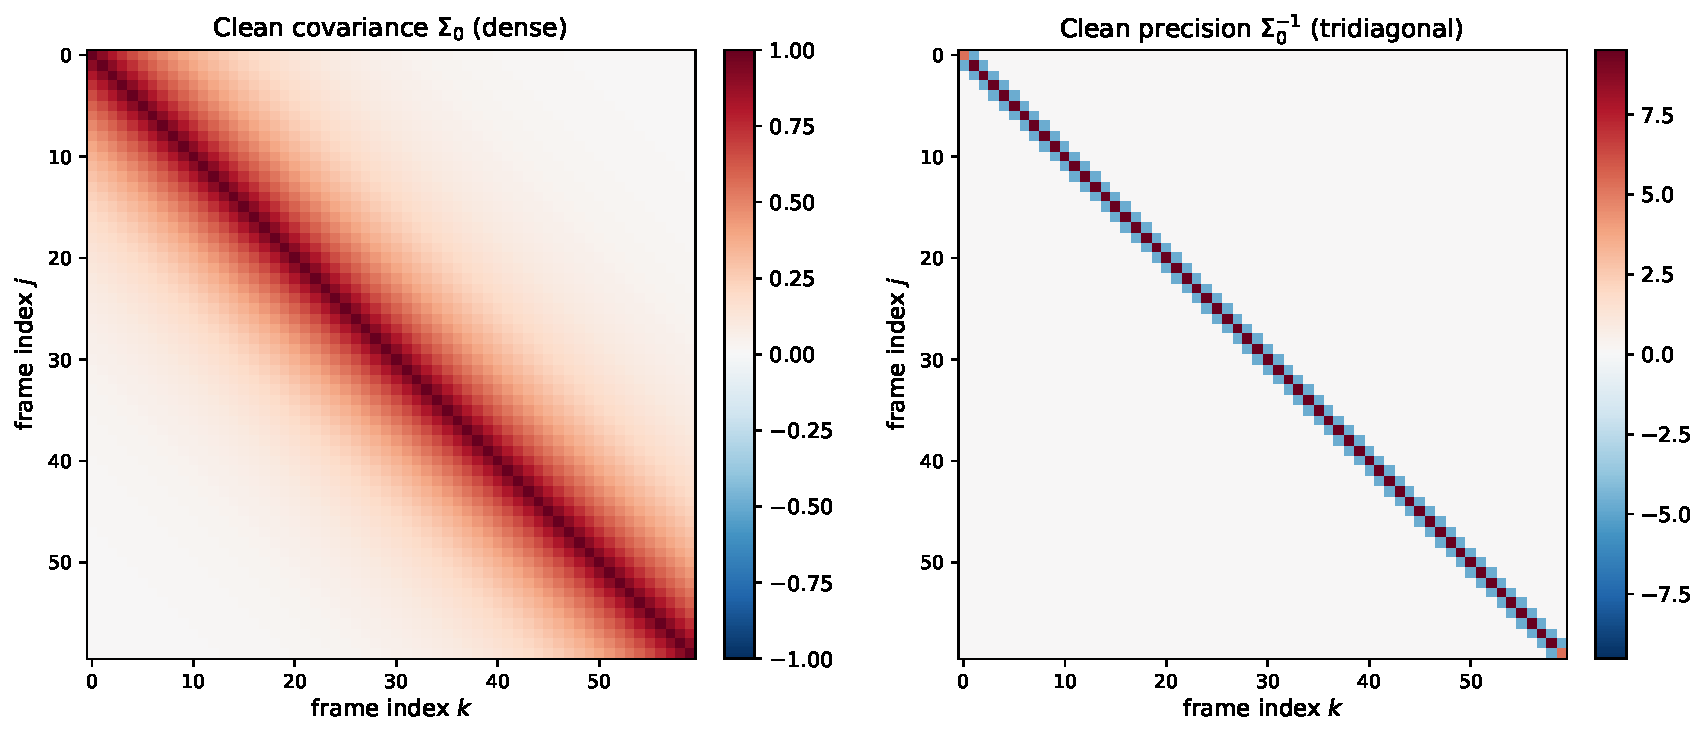
\includegraphics[width=.93\textwidth]{figures/fig01_sigma0_vs_precision0.pdf}
\caption{Clean covariance versus clean precision. The covariance matrix is dense because every frame is marginally correlated with every other frame. The precision matrix is tridiagonal because the conditional dependence structure is local: once neighbors are known, more distant frames do not enter the conditional mean.}
\label{fig:sigma0_prec0}
\end{figure}

\begin{figure}[H]
\centering
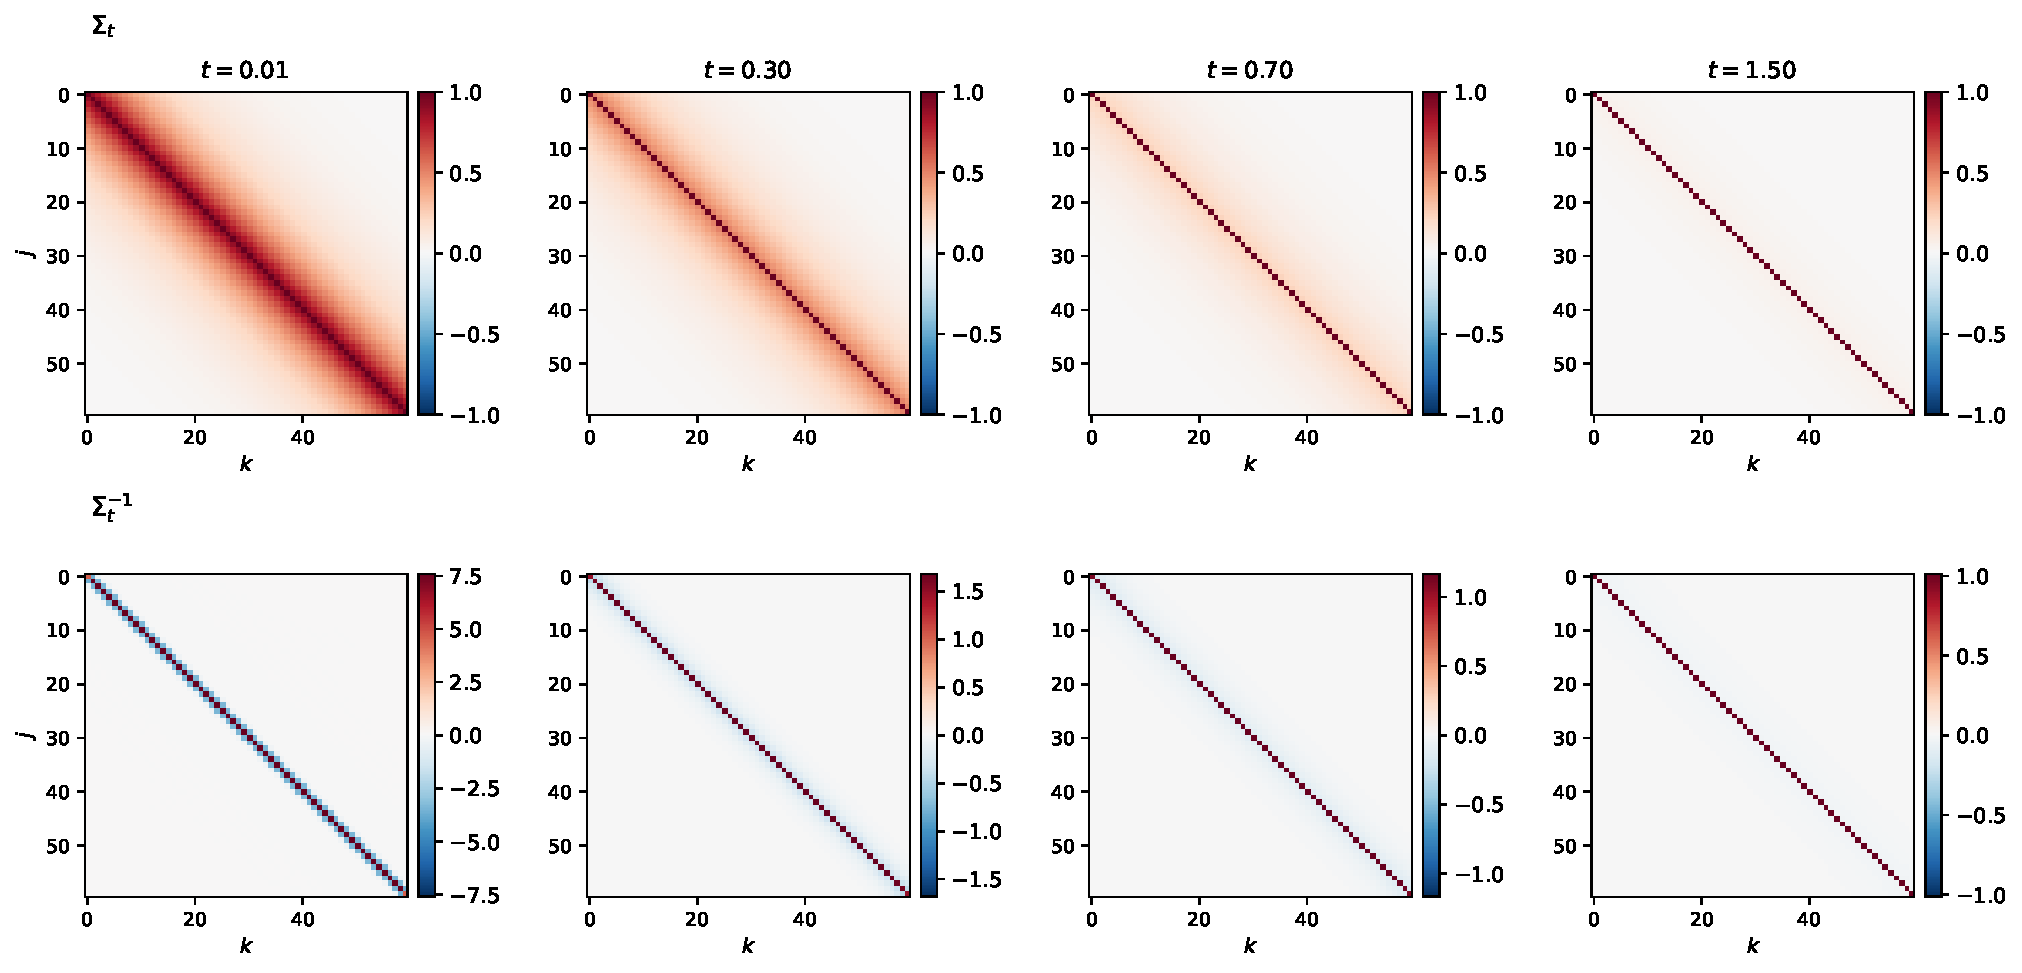
\includegraphics[width=.97\textwidth]{figures/fig02_sigma_t_panel.pdf}
\caption{Evolution of the covariance $\Sigma_t$ and precision $\Sigma_t^{-1}$ as diffusion time increases. The covariance moves steadily toward the identity. The precision starts from the tridiagonal clean precision, then becomes full for $t>0$, and finally approaches the identity in the pure-noise limit.}
\label{fig:sigmat_panel}
\end{figure}

\begin{figure}[H]
\centering
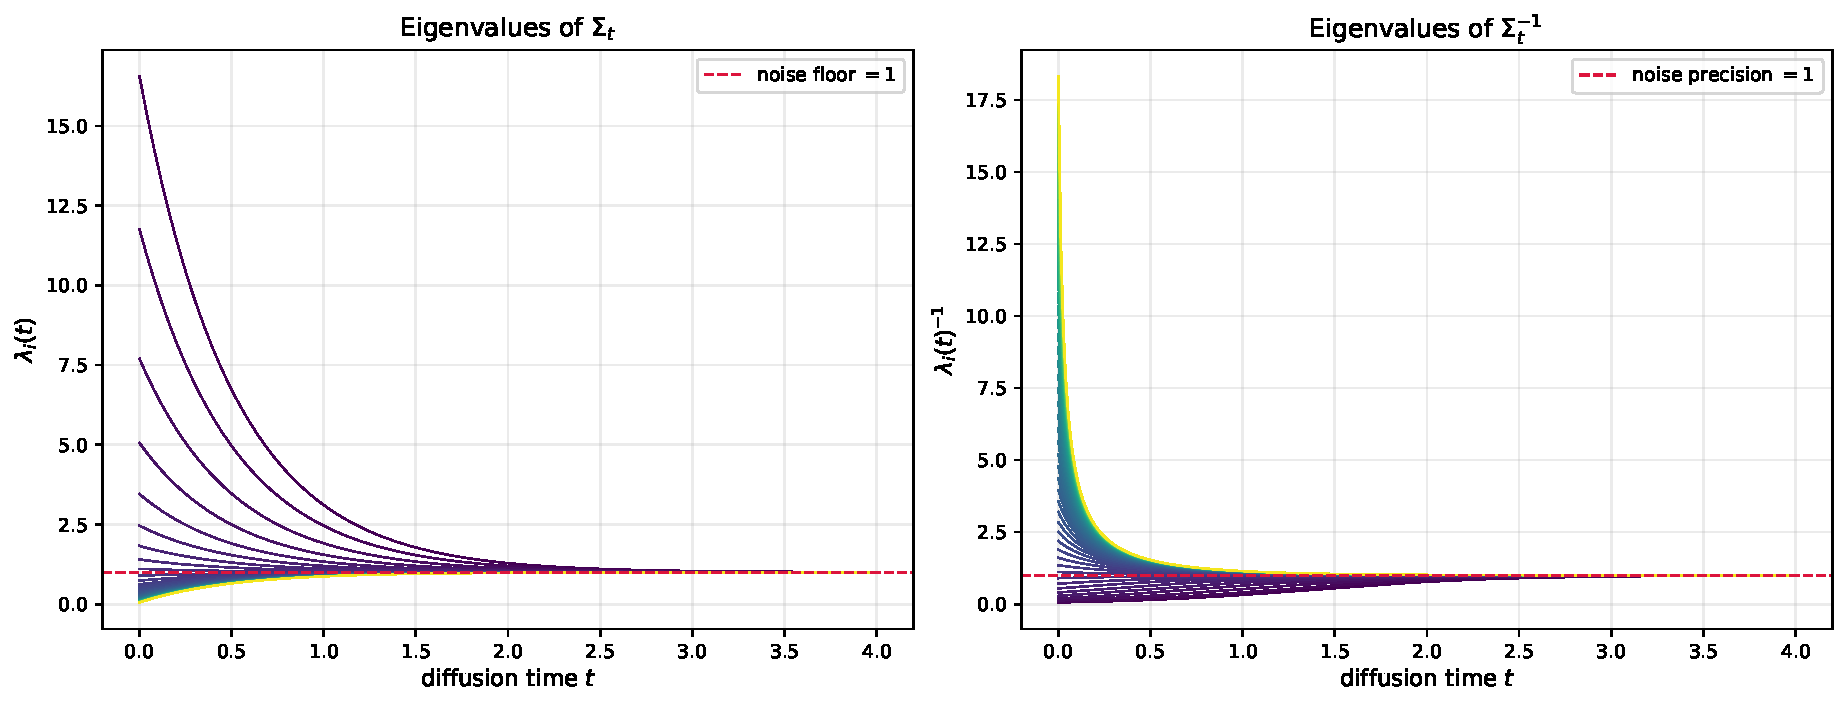
\includegraphics[width=.93\textwidth]{figures/fig03_eigenvalue_trajectories.pdf}
\caption{Eigenvalue dynamics. Left: the eigenvalues of $\Sigma_t$ evolve according to $\lambda_i(t)=e^{-2t}\lambda_i+\Delta_t$ and all drift toward $1$. Right: the eigenvalues of $\Sigma_t^{-1}$ also flatten toward $1$. The spectrum contracts toward the isotropic noise spectrum.}
\label{fig:eigtraj}
\end{figure}

\begin{figure}[H]
\centering
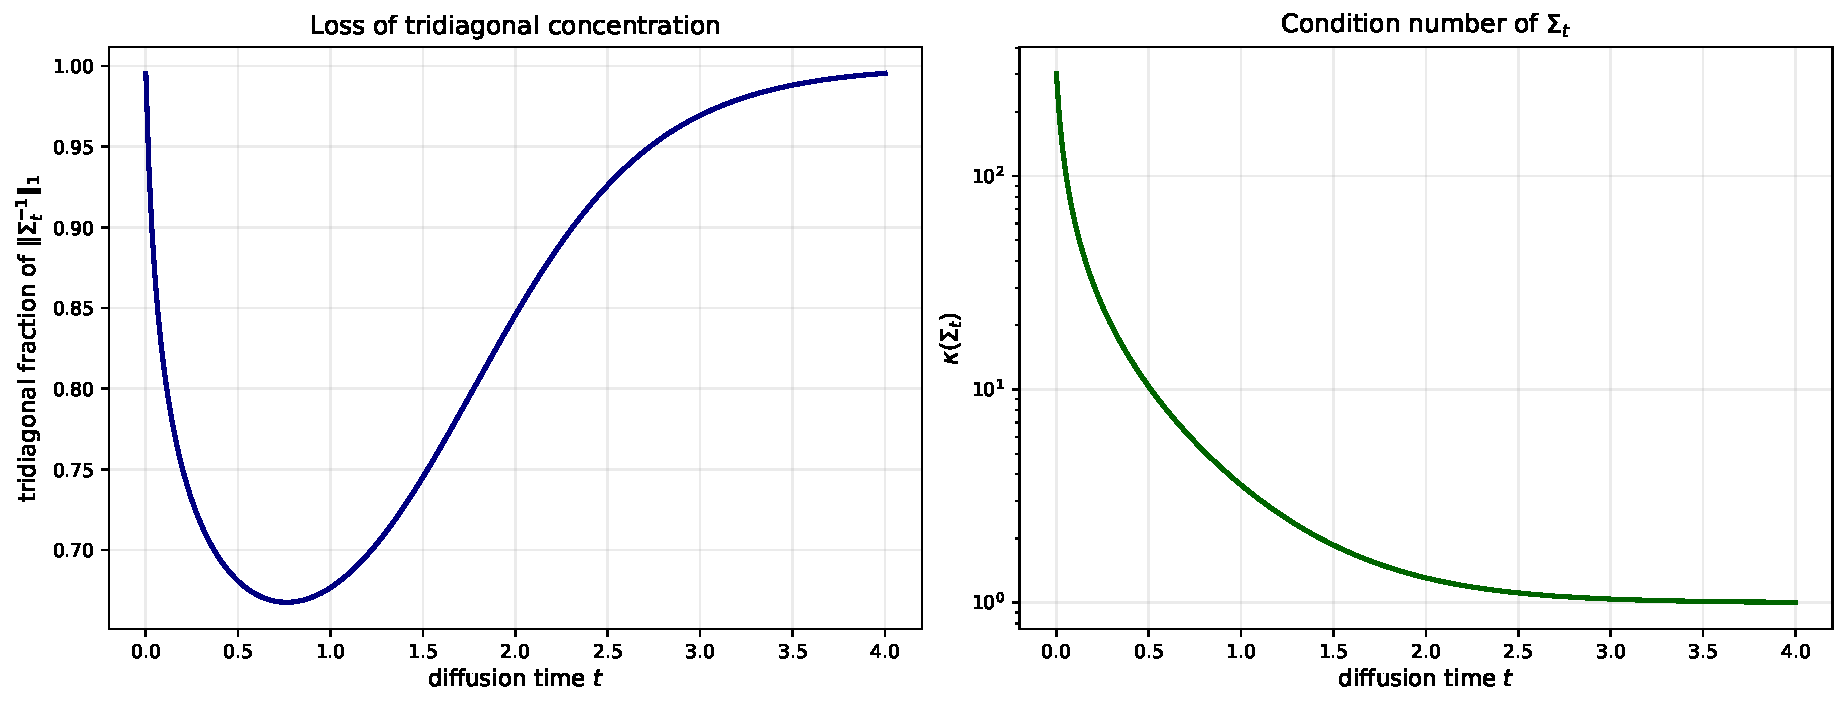
\includegraphics[width=.93\textwidth]{figures/fig04_tridiag_fraction_condition.pdf}
\caption{Left: the fraction of the entrywise $\ell_1$ mass of $\Sigma_t^{-1}$ located on the tridiagonal band decreases with $t$, quantifying the loss of Markov-local structure in the frame basis. Right: the condition number of $\Sigma_t$ decreases toward $1$, indicating that diffusion improves numerical conditioning.}
\label{fig:tridiag_condition}
\end{figure}

\begin{figure}[H]
\centering
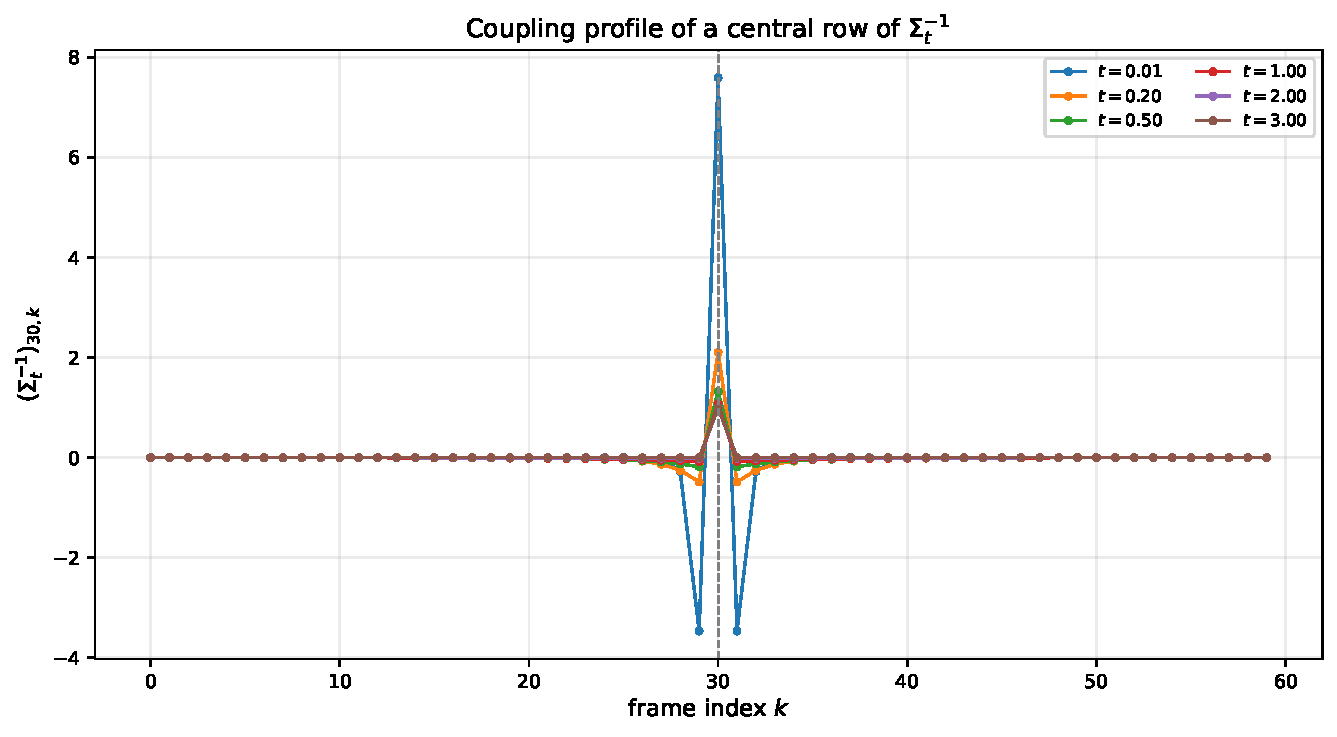
\includegraphics[width=.72\textwidth]{figures/fig05_precision_row_profile.pdf}
\caption{A central row of the noisy precision matrix for several diffusion times. At $t\approx 0$ the row is concentrated on the diagonal and its nearest neighbors. As diffusion increases, coupling spreads to distant frames and eventually contracts again toward the identity profile.}
\label{fig:rowprofile}
\end{figure}

\begin{figure}[H]
\centering
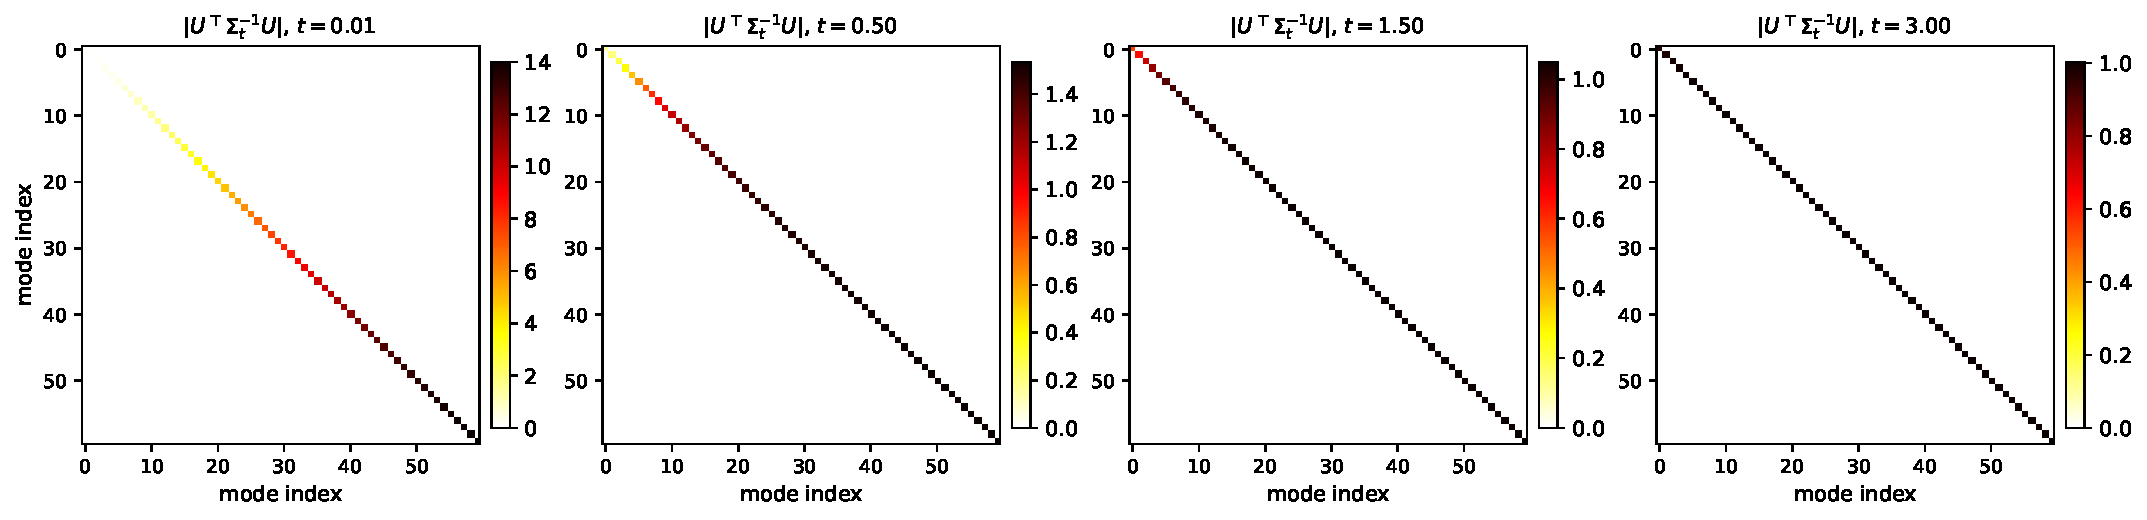
\includegraphics[width=.93\textwidth]{figures/fig06_precision_eigenbasis.pdf}
\caption{Absolute value of $U^\trans\Sigma_t^{-1}U$ for several diffusion times. The near-perfect diagonality confirms the exact spectral decoupling: in the eigenbasis of $\Sigma_0$, the precision matrix remains diagonal for all $t$.}
\label{fig:eigenbasis}
\end{figure}

\begin{figure}[H]
\centering
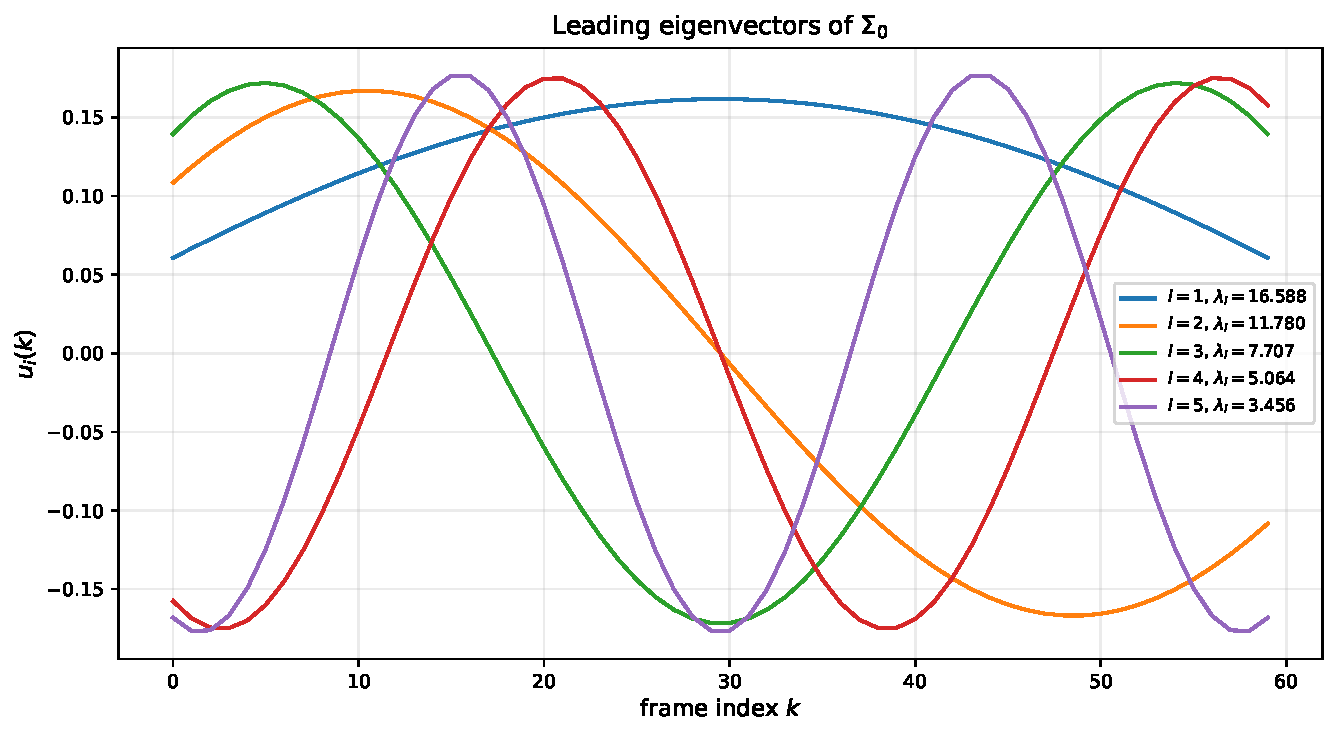
\includegraphics[width=.72\textwidth]{figures/fig07_eigenvectors.pdf}
\caption{Leading eigenvectors of the clean covariance. In the stationary AR(1) regime they resemble smooth discrete oscillatory modes. These vectors define the orthogonal change of coordinates that turns the correlated frame basis into a basis of independent Gaussian modes.}
\label{fig:eigvecs}
\end{figure}

\subsection{Interpretation of the numerical study}

The numerical experiments illustrate every structural claim proved in the previous sections.

First, \Cref{fig:sigma0_prec0} visualizes the clean contrast between covariance and precision: dense marginal correlations versus sparse conditional couplings.

Second, \Cref{fig:sigmat_panel,fig:rowprofile} show the geometric effect of diffusion in the original frame basis. The covariance moves toward the identity, while the precision loses its exact tridiagonal sparsity and becomes full as soon as isotropic noise is added.

Third, \Cref{fig:eigtraj} confirms the spectral formulas derived in \Cref{sec:sigmat}: every eigenvalue follows an explicit scalar interpolation between its clean value and the noise floor $1$.

Fourth, \Cref{fig:eigenbasis} gives the core structural message of the manuscript: what looks complicated in the frame basis becomes exactly diagonal in the eigenbasis. The full multivariate denoising problem is therefore a collection of independent scalar Gaussian problems.

Finally, \Cref{fig:tridiag_condition} shows two complementary trends: diffusion degrades locality in the frame basis while simultaneously improving conditioning and thus simplifying inversion and optimization in spectral space.

\section{Conclusion}

The AR(1) diffusion model is simple enough to solve exactly and rich enough to display the essential structural phenomena behind diffusion on correlated sequences.

The clean process is Gaussian and Markov. Gaussianity determines that the whole law is encoded by a covariance matrix. Markovianity determines that the inverse covariance, not the covariance itself, is local: the clean precision matrix is tridiagonal. This already separates marginal correlation from direct conditional dependence.

The forward diffusion process adds independent Ornstein--Uhlenbeck noise to each frame. Because the noising map is affine and all ingredients are Gaussian, the noisy law remains Gaussian. Its covariance takes the explicit form
\[
\Sigma_t=e^{-2t}\Sigma_0+\Delta_t\Id.
\]
This formula separates the surviving clean signal covariance from the isotropic noise floor.

From there, the score follows immediately:
\[
S(\mathbf x,t)=-\Sigma_t^{-1}(\mathbf x-\boldsymbol{\mu}_t).
\]
Hence all structural questions about the score reduce to understanding the precision matrix. In the original frame basis, diffusion destroys exact tridiagonality and fills in long-range couplings. In the eigenbasis of the clean covariance, however, the situation becomes completely transparent. The eigenvectors stay fixed for all diffusion times, the eigenvalues evolve according to
\[
\lambda_i(t)=e^{-2t}\lambda_i+\Delta_t,
\]
and the score decouples into independent scalar denoisers
\[
\widetilde S_i(\widetilde{\mathbf x},t)
=
-\frac{\widetilde x_i-\widetilde\mu_{t,i}}{e^{-2t}\lambda_i+\Delta_t}.
\]

This makes the central structural distinction precise:
\begin{itemize}[leftmargin=1cm]
\item Gaussianity enables complete decoupling once the covariance is diagonalized.
\item Markovianity shapes the particular spectrum and eigenvectors that are being diagonalized.
\end{itemize}

The resulting picture is mathematically clean and conceptually useful. Diffusion progressively erases anisotropy and local structure in the frame basis, yet reveals perfect independence in the spectral basis. That duality is the central lesson of the model.

\begin{thebibliography}{99}

\bibitem{draftar1}
G.~Mantovani and M.~Lomel\'e.
\newblock \emph{Joint Score of a Diffusion Model Applied to an AR(1) Sequence: A Self-Contained Derivation}.
\newblock MSc thesis notes, Bocconi University, 2025--2026.

\bibitem{structure}
G.~Mantovani and M.~Lomel\'e.
\newblock \emph{The Structure of $\Sigma_t$ and $\Sigma_t^{-1}$ in the AR(1) Diffusion Model: Explicit Inversion, Spectral Decomposition, and Numerical Study}.
\newblock MSc thesis notes, Bocconi University, March 2026.

\bibitem{anatomy}
G.~Mantovani and M.~Lomel\'e.
\newblock \emph{The Anatomy of $\Sigma_t$ and $\Sigma_t^{-1}$: How Diffusion Noise Reshapes the Score of an AR(1) Sequence}.
\newblock MSc thesis notes, Bocconi University, March 2026.

\bibitem{companion}
G.~Mantovani and M.~Lomel\'e.
\newblock \emph{Mathematical Companion: Deep-Dive Explanations for the $\Sigma_t$ Analysis}.
\newblock MSc thesis notes, Bocconi University, March 2026.

\bibitem{mezardnotes}
M.~M\'ezard.
\newblock \emph{Generative Diffusion Updated Notes}.
\newblock Lecture notes, December 2025.

\bibitem{biroli2023}
G.~Biroli and M.~M\'ezard.
\newblock Generative diffusion in very large dimensions.
\newblock \emph{arXiv preprint arXiv:2306.03518}, 2023.

\end{thebibliography}

\end{document}
